\documentclass[11pt]{report}
\usepackage{./assignment_programming}
\usepackage{slashbox}
\usepackage{enumerate}
\usepackage[shortlabels]{enumitem}
\usepackage{stmaryrd}
\usepackage{graphicx}
\usepackage[final]{pdfpages}
\usepackage{array}
\usepackage{multirow}
\usepackage{subfigure}
%\PassOptionsToPackage{normalem}{ulem}
%\usepackage{ulem}

\RequirePackage{latexsym}
\RequirePackage{amsmath}
\RequirePackage{amssymb}
\RequirePackage{bm}
\RequirePackage{url}
\RequirePackage{algorithmic}
\RequirePackage{algorithm2e}


%%%%%%%% Stock standard definitions %%%%%%%%%%%%%%%

%\newcommand{\ab}{\mathbf{a}}
%\newcommand{\bb}{\mathbf{b}}
%\newcommand{\cbb}{\mathbf{c}}
%\newcommand{\db}{\mathbf{d}}
%\newcommand{\eb}{\mathbf{e}}
%\newcommand{\fb}{\mathbf{f}}
%\newcommand{\gb}{\mathbf{g}}
%\newcommand{\hb}{\mathbf{h}}
%\newcommand{\ib}{\mathbf{i}}
%\newcommand{\jb}{\mathbf{j}}
%\newcommand{\kb}{\mathbf{k}}
%\newcommand{\lb}{\mathbf{l}}
%\newcommand{\mb}{\mathbf{m}}
%\newcommand{\nbb}{\mathbf{n}}
%\newcommand{\ob}{\mathbf{o}}
%\newcommand{\pb}{\mathbf{p}}
%\newcommand{\qb}{\mathbf{q}}
%\newcommand{\rb}{\mathbf{r}}
%\newcommand{\sbb}{\mathbf{s}}
%\newcommand{\tb}{\mathbf{t}}
%\newcommand{\ub}{\mathbf{u}}
%\newcommand{\vb}{\mathbf{v}}
%\newcommand{\wb}{\mathbf{w}}
%\newcommand{\xb}{\mathbf{x}}
%\newcommand{\yb}{\mathbf{y}}
%\newcommand{\zb}{\mathbf{z}}
%
%\newcommand{\abtil}{\tilde{\ab}}
%\newcommand{\bbtil}{\tilde{\bb}}
%\newcommand{\cbtil}{\tilde{\cbb}}
%\newcommand{\dbtil}{\tilde{\db}}
%\newcommand{\ebtil}{\tilde{\eb}}
%\newcommand{\fbtil}{\tilde{\fb}}
%\newcommand{\gbtil}{\tilde{\gb}}
%\newcommand{\hbtil}{\tilde{\hb}}
%\newcommand{\ibtil}{\tilde{\ib}}
%\newcommand{\jbtil}{\tilde{\jb}}
%\newcommand{\kbtil}{\tilde{\kb}}
%\newcommand{\lbtil}{\tilde{\lb}}
%\newcommand{\mbtil}{\tilde{\mb}}
%\newcommand{\nbtil}{\tilde{\nbb}}
%\newcommand{\obtil}{\tilde{\ob}}
%\newcommand{\pbtil}{\tilde{\pb}}
%\newcommand{\qbtil}{\tilde{\qb}}
%\newcommand{\rbtil}{\tilde{\rb}}
%\newcommand{\sbtil}{\tilde{\sbb}}
%\newcommand{\tbtil}{\tilde{\tb}}
%\newcommand{\ubtil}{\tilde{\ub}}
%\newcommand{\vbtil}{\tilde{\vb}}
%\newcommand{\wbtil}{\tilde{\wb}}
%\newcommand{\xbtil}{\tilde{\xb}}
%\newcommand{\ybtil}{\tilde{\yb}}
%\newcommand{\zbtil}{\tilde{\zb}}
%
%
%\newcommand{\atil}{\tilde{a}}
%\newcommand{\btil}{\tilde{b}}
%\newcommand{\ctil}{\tilde{c}}
%\newcommand{\dtil}{\tilde{d}}
%\newcommand{\etil}{\tilde{e}}
%\newcommand{\ftil}{\tilde{f}}
%\newcommand{\gtil}{\tilde{g}}
%\newcommand{\htil}{\tilde{h}}
%\newcommand{\itil}{\tilde{i}}
%\newcommand{\jtil}{\tilde{j}}
%\newcommand{\ktil}{\tilde{k}}
%\newcommand{\ltil}{\tilde{l}}
%\newcommand{\mtil}{\tilde{m}}
%\newcommand{\ntil}{\tilde{n}}
%\newcommand{\otil}{\tilde{o}}
%\newcommand{\ptil}{\tilde{p}}
%\newcommand{\qtil}{\tilde{q}}
%\newcommand{\rtil}{\tilde{r}}
%\newcommand{\stil}{\tilde{s}}
%\newcommand{\ttil}{\tilde{t}}
%\newcommand{\util}{\tilde{u}}
%\newcommand{\vtil}{\tilde{v}}
%\newcommand{\wtil}{\tilde{w}}
%\newcommand{\xtil}{\tilde{x}}
%\newcommand{\ytil}{\tilde{y}}
%\newcommand{\ztil}{\tilde{z}}
%
%\newcommand{\Atil}{\tilde{A}}
%\newcommand{\Btil}{\tilde{B}}
%\newcommand{\Ctil}{\tilde{C}}
%\newcommand{\Dtil}{\tilde{D}}
%\newcommand{\Etil}{\tilde{E}}
%\newcommand{\Ftil}{\tilde{F}}
%\newcommand{\Gtil}{\tilde{G}}
%\newcommand{\Htil}{\tilde{H}}
%\newcommand{\Itil}{\tilde{I}}
%\newcommand{\Jtil}{\tilde{J}}
%\newcommand{\Ktil}{\tilde{K}}
%\newcommand{\Ltil}{\tilde{L}}
%\newcommand{\Mtil}{\tilde{M}}
%\newcommand{\Ntil}{\tilde{N}}
%\newcommand{\Otil}{\tilde{O}}
%\newcommand{\Ptil}{\tilde{P}}
%\newcommand{\Qtil}{\tilde{Q}}
%\newcommand{\Rtil}{\tilde{R}}
%\newcommand{\Stil}{\tilde{S}}
%\newcommand{\Ttil}{\tilde{T}}
%\newcommand{\Util}{\tilde{U}}
%\newcommand{\Vtil}{\tilde{V}}
%\newcommand{\Wtil}{\tilde{W}}
%\newcommand{\Xtil}{\tilde{X}}
%\newcommand{\Ytil}{\tilde{Y}}
%\newcommand{\Ztil}{\tilde{Z}}
%
%\newcommand{\abar}{\bar{a}}
%\newcommand{\bbar}{\bar{b}}
%\newcommand{\cbar}{\bar{c}}
%\newcommand{\dbar}{\bar{d}}
%\newcommand{\ebar}{\bar{e}}
%\newcommand{\fbar}{\bar{f}}
%\newcommand{\gbar}{\bar{g}}
%\newcommand{\hbr}{\bar{h}}
%\newcommand{\ibar}{\bar{i}}
%\newcommand{\jbar}{\bar{j}}
%\newcommand{\kbar}{\bar{k}}
%\newcommand{\lbar}{\bar{l}}
%\newcommand{\mbar}{\bar{m}}
%\newcommand{\nbar}{\bar{n}}
%\newcommand{\obar}{\bar{o}}
%\newcommand{\pbar}{\bar{p}}
%\newcommand{\qbar}{\bar{q}}
%\newcommand{\rbar}{\bar{r}}
%\newcommand{\sbar}{\bar{s}}
%\newcommand{\tbar}{\bar{t}}
%\newcommand{\ubar}{\bar{u}}
%\newcommand{\vbar}{\bar{v}}
%\newcommand{\wbar}{\bar{w}}
%\newcommand{\xbar}{\bar{x}}
%\newcommand{\ybar}{\bar{y}}
%\newcommand{\zbar}{\bar{z}}
%
%\newcommand{\abbar}{\bar{\ab}}
%\newcommand{\bbbar}{\bar{\bb}}
%\newcommand{\cbbar}{\bar{\cb}}
%\newcommand{\dbbar}{\bar{\db}}
%\newcommand{\ebbar}{\bar{\eb}}
%\newcommand{\fbbar}{\bar{\fb}}
%\newcommand{\gbbar}{\bar{\gb}}
%\newcommand{\hbbar}{\bar{\hb}}
%\newcommand{\ibbar}{\bar{\ib}}
%\newcommand{\jbbar}{\bar{\jb}}
%\newcommand{\kbbar}{\bar{\kb}}
%\newcommand{\lbbar}{\bar{\lb}}
%\newcommand{\mbbar}{\bar{\mb}}
%\newcommand{\nbbar}{\bar{\nbb}}
%\newcommand{\obbar}{\bar{\ob}}
%\newcommand{\pbbar}{\bar{\pb}}
%\newcommand{\qbbar}{\bar{\qb}}
%\newcommand{\rbbar}{\bar{\rb}}
%\newcommand{\sbbar}{\bar{\sbb}}
%\newcommand{\tbbar}{\bar{\tb}}
%\newcommand{\ubbar}{\bar{\ub}}
%\newcommand{\vbbar}{\bar{\vb}}
%\newcommand{\wbbar}{\bar{\wb}}
%\newcommand{\xbbar}{\bar{\xb}}
%\newcommand{\ybbar}{\bar{\yb}}
%\newcommand{\zbbar}{\bar{\zb}}
%
%\newcommand{\Ab}{\mathbf{A}}
%\newcommand{\Bb}{\mathbf{B}}
%\newcommand{\Cb}{\mathbf{C}}
%\newcommand{\Db}{\mathbf{D}}
%\newcommand{\Eb}{\mathbf{E}}
%\newcommand{\Fb}{\mathbf{F}}
%\newcommand{\Gb}{\mathbf{G}}
%\newcommand{\Hb}{\mathbf{H}}
%\newcommand{\Ib}{\mathbf{I}}
%\newcommand{\Jb}{\mathbf{J}}
%\newcommand{\Kb}{\mathbf{K}}
%\newcommand{\Lb}{\mathbf{L}}
%\newcommand{\Mb}{\mathbf{M}}
%\newcommand{\Nb}{\mathbf{N}}
%\newcommand{\Ob}{\mathbf{O}}
%\newcommand{\Pb}{\mathbf{P}}
%\newcommand{\Qb}{\mathbf{Q}}
%\newcommand{\Rb}{\mathbf{R}}
%\newcommand{\Sbb}{\mathbf{S}}
%\newcommand{\Tb}{\mathbf{T}}
%\newcommand{\Ub}{\mathbf{U}}
%\newcommand{\Vb}{\mathbf{V}}
%\newcommand{\Wb}{\mathbf{W}}
%\newcommand{\Xb}{\mathbf{X}}
%\newcommand{\Yb}{\mathbf{Y}}
%\newcommand{\Zb}{\mathbf{Z}}
%
%\newcommand{\Abtil}{\tilde{\Ab}}
%\newcommand{\Bbtil}{\tilde{\Bb}}
%\newcommand{\Cbtil}{\tilde{\Cb}}
%\newcommand{\Dbtil}{\tilde{\Db}}
%\newcommand{\Ebtil}{\tilde{\Eb}}
%\newcommand{\Fbtil}{\tilde{\Fb}}
%\newcommand{\Gbtil}{\tilde{\Gb}}
%\newcommand{\Hbtil}{\tilde{\Hb}}
%\newcommand{\Ibtil}{\tilde{\Ib}}
%\newcommand{\Jbtil}{\tilde{\Jb}}
%\newcommand{\Kbtil}{\tilde{\Kb}}
%\newcommand{\Lbtil}{\tilde{\Lb}}
%\newcommand{\Mbtil}{\tilde{\Mb}}
%\newcommand{\Nbtil}{\tilde{\Nb}}
%\newcommand{\Obtil}{\tilde{\Ob}}
%\newcommand{\Pbtil}{\tilde{\Pb}}
%\newcommand{\Qbtil}{\tilde{\Qb}}
%\newcommand{\Rbtil}{\tilde{\Rb}}
%\newcommand{\Sbtil}{\tilde{\Sbb}}
%\newcommand{\Tbtil}{\tilde{\Tb}}
%\newcommand{\Ubtil}{\tilde{\Ub}}
%\newcommand{\Vbtil}{\tilde{\Vb}}
%\newcommand{\Wbtil}{\tilde{\Wb}}
%\newcommand{\Xbtil}{\tilde{\Xb}}
%\newcommand{\Ybtil}{\tilde{\Yb}}
%\newcommand{\Zbtil}{\tilde{\Zb}}
%
%\newcommand{\Abar}{\bar{A}}
%\newcommand{\Bbar}{\bar{B}}
%\newcommand{\Cbar}{\bar{C}}
%\newcommand{\Dbar}{\bar{D}}
%\newcommand{\Ebar}{\bar{E}}
%\newcommand{\Fbar}{\bar{F}}
%\newcommand{\Gbar}{\bar{G}}
%\newcommand{\Hbar}{\bar{H}}
%\newcommand{\Ibar}{\bar{I}}
%\newcommand{\Jbar}{\bar{J}}
%\newcommand{\Kbar}{\bar{K}}
%\newcommand{\Lbar}{\bar{L}}
%\newcommand{\Mbar}{\bar{M}}
%\newcommand{\Nbar}{\bar{N}}
%\newcommand{\Obar}{\bar{O}}
%\newcommand{\Pbar}{\bar{P}}
%\newcommand{\Qbar}{\bar{Q}}
%\newcommand{\Rbar}{\bar{R}}
%\newcommand{\Sbar}{\bar{S}}
%\newcommand{\Tbar}{\bar{T}}
%\newcommand{\Ubar}{\bar{U}}
%\newcommand{\Vbar}{\bar{V}}
%\newcommand{\Wbar}{\bar{W}}
%\newcommand{\Xbar}{\bar{X}}
%\newcommand{\Ybar}{\bar{Y}}
%\newcommand{\Zbar}{\bar{Z}}
%
%\newcommand{\Abbar}{\bar{\Ab}}
%\newcommand{\Bbbar}{\bar{\Bb}}
%\newcommand{\Cbbar}{\bar{\Cb}}
%\newcommand{\Dbbar}{\bar{\Db}}
%\newcommand{\Ebbar}{\bar{\Eb}}
%\newcommand{\Fbbar}{\bar{\Fb}}
%\newcommand{\Gbbar}{\bar{\Gb}}
%\newcommand{\Hbbar}{\bar{\Hb}}
%\newcommand{\Ibbar}{\bar{\Ib}}
%\newcommand{\Jbbar}{\bar{\Jb}}
%\newcommand{\Kbbar}{\bar{\Kb}}
%\newcommand{\Lbbar}{\bar{\Lb}}
%\newcommand{\Mbbar}{\bar{\Mb}}
%\newcommand{\Nbbar}{\bar{\Nb}}
%\newcommand{\Obbar}{\bar{\Ob}}
%\newcommand{\Pbbar}{\bar{\Pb}}
%\newcommand{\Qbbar}{\bar{\Qb}}
%\newcommand{\Rbbar}{\bar{\Rb}}
%\newcommand{\Sbbar}{\bar{\Sb}}
%\newcommand{\Tbbar}{\bar{\Tb}}
%\newcommand{\Ubbar}{\bar{\Ub}}
%\newcommand{\Vbbar}{\bar{\Vb}}
%\newcommand{\Wbbar}{\bar{\Wb}}
%\newcommand{\Xbbar}{\bar{\Xb}}
%\newcommand{\Ybbar}{\bar{\Yb}}
%\newcommand{\Zbbar}{\bar{\Zb}}
%
%\newcommand{\Ahat}{\hat{A}}
%\newcommand{\Bhat}{\hat{B}}
%\newcommand{\Chat}{\hat{C}}
%\newcommand{\Dhat}{\hat{D}}
%\newcommand{\Ehat}{\hat{E}}
%\newcommand{\Fhat}{\hat{F}}
%\newcommand{\Ghat}{\hat{G}}
%\newcommand{\Hhat}{\hat{H}}
%\newcommand{\Ihat}{\hat{I}}
%\newcommand{\Jhat}{\hat{J}}
%\newcommand{\Khat}{\hat{K}}
%\newcommand{\Lhat}{\hat{L}}
%\newcommand{\Mhat}{\hat{M}}
%\newcommand{\Nhat}{\hat{N}}
%\newcommand{\Ohat}{\hat{O}}
%\newcommand{\Phat}{\hat{P}}
%\newcommand{\Qhat}{\hat{Q}}
%\newcommand{\Rhat}{\hat{R}}
%\newcommand{\Shat}{\hat{S}}
%\newcommand{\That}{\hat{T}}
%\newcommand{\Uhat}{\hat{U}}
%\newcommand{\Vhat}{\hat{V}}
%\newcommand{\What}{\hat{W}}
%\newcommand{\Xhat}{\hat{X}}
%\newcommand{\Yhat}{\hat{Y}}
%\newcommand{\Zhat}{\hat{Z}}
%
%\newcommand{\Abhat}{\hat{\Ab}}
%\newcommand{\Bbhat}{\hat{\Bb}}
%\newcommand{\Cbhat}{\hat{\Cb}}
%\newcommand{\Dbhat}{\hat{\Db}}
%\newcommand{\Ebhat}{\hat{\Eb}}
%\newcommand{\Fbhat}{\hat{\Fb}}
%\newcommand{\Gbhat}{\hat{\Gb}}
%\newcommand{\Hbhat}{\hat{\Hb}}
%\newcommand{\Ibhat}{\hat{\Ib}}
%\newcommand{\Jbhat}{\hat{\Jb}}
%\newcommand{\Kbhat}{\hat{\Kb}}
%\newcommand{\Lbhat}{\hat{\Lb}}
%\newcommand{\Mbhat}{\hat{\Mb}}
%\newcommand{\Nbhat}{\hat{\Nb}}
%\newcommand{\Obhat}{\hat{\Ob}}
%\newcommand{\Pbhat}{\hat{\Pb}}
%\newcommand{\Qbhat}{\hat{\Qb}}
%\newcommand{\Rbhat}{\hat{\Rb}}
%\newcommand{\Sbhat}{\hat{\Sb}}
%\newcommand{\Tbhat}{\hat{\Tb}}
%\newcommand{\Ubhat}{\hat{\Ub}}
%\newcommand{\Vbhat}{\hat{\Vb}}
%\newcommand{\Wbhat}{\hat{\Wb}}
%\newcommand{\Xbhat}{\hat{\Xb}}
%\newcommand{\Ybhat}{\hat{\Yb}}
%\newcommand{\Zbhat}{\hat{\Zb}}
%
%\newcommand{\Acal}{\mathcal{A}}
%\newcommand{\Bcal}{\mathcal{B}}
%\newcommand{\Ccal}{\mathcal{C}}
%\newcommand{\Dcal}{\mathcal{D}}
%\newcommand{\Ecal}{\mathcal{E}}
%\newcommand{\Fcal}{\mathcal{F}}
%\newcommand{\Gcal}{\mathcal{G}}
%\newcommand{\Hcal}{\mathcal{H}}
%\newcommand{\Ical}{\mathcal{I}}
%\newcommand{\Jcal}{\mathcal{J}}
%\newcommand{\Kcal}{\mathcal{K}}
%\newcommand{\Lcal}{\mathcal{L}}
%\newcommand{\Mcal}{\mathcal{M}}
%\newcommand{\Ncal}{\mathcal{N}}
%\newcommand{\Ocal}{\mathcal{O}}
%\newcommand{\Pcal}{\mathcal{P}}
%\newcommand{\Qcal}{\mathcal{Q}}
%\newcommand{\Rcal}{\mathcal{R}}
%\newcommand{\Scal}{{\mathcal{S}}}
%\newcommand{\Tcal}{{\mathcal{T}}}
%\newcommand{\Ucal}{\mathcal{U}}
%\newcommand{\Vcal}{\mathcal{V}}
%\newcommand{\Wcal}{\mathcal{W}}
%\newcommand{\Xcal}{\mathcal{X}}
%\newcommand{\Ycal}{\mathcal{Y}}
%\newcommand{\Zcal}{\mathcal{Z}}
%
%\newcommand{\Atilde}{\widetilde{A}}
%\newcommand{\Btilde}{\widetilde{B}}
%\newcommand{\Ctilde}{\widetilde{C}}
%\newcommand{\Dtilde}{\widetilde{D}}
%\newcommand{\Etilde}{\widetilde{E}}
%\newcommand{\Ftilde}{\widetilde{F}}
%\newcommand{\Gtilde}{\widetilde{G}}
%\newcommand{\Htilde}{\widetilde{H}}
%\newcommand{\Itilde}{\widetilde{I}}
%\newcommand{\Jtilde}{\widetilde{J}}
%\newcommand{\Ktilde}{\widetilde{K}}
%\newcommand{\Ltilde}{\widetilde{L}}
%\newcommand{\Mtilde}{\widetilde{M}}
%\newcommand{\Ntilde}{\widetilde{N}}
%\newcommand{\Otilde}{\widetilde{O}}
%\newcommand{\Ptilde}{\widetilde{P}}
%\newcommand{\Qtilde}{\widetilde{Q}}
%\newcommand{\Rtilde}{\widetilde{R}}
%\newcommand{\Stilde}{\widetilde{S}}
%\newcommand{\Ttilde}{\widetilde{T}}
%\newcommand{\Utilde}{\widetilde{U}}
%\newcommand{\Vtilde}{\widetilde{V}}
%\newcommand{\Wtilde}{\widetilde{W}}
%\newcommand{\Xtilde}{\widetilde{X}}
%\newcommand{\Ytilde}{\widetilde{Y}}
%\newcommand{\Ztilde}{\widetilde{Z}}
%
%
%%%%%%%%% Widely accepted definitions %%%%%%%%%%%%%%%
%
%\newcommand{\CC}{\mathbb{C}} % Complex numbers
%\newcommand{\EE}{\mathbb{E}} % Expectation
%\newcommand{\II}{\mathbb{I}} % Delta Indicator
%\newcommand{\VV}{\mathbb{V}} % Variance
%\newcommand{\KK}{\mathbb{K}} % Arbitrary field
%\newcommand{\MM}{\mathbb{M}} % Median
%\newcommand{\NN}{\mathbb{N}} % Natural numbers
%\newcommand{\PP}{\mathbb{P}} % Probability
%\newcommand{\QQ}{\mathbb{Q}} % Rationals
%\newcommand{\RR}{\mathbb{R}} % Real numbers
%\newcommand{\ZZ}{\mathbb{Z}} % Integers
%\newcommand{\XX}{\mathbb{X}} % Integers
%\newcommand{\YY}{\mathbb{Y}} % Integers
%
%\newcommand{\one}{\mathbf{1}}  % Identity
%\newcommand{\zero}{\mathbf{0}} % Zero
%%\newcommand{\TRUE}{\mathbf{TRUE}}  % True
%%\newcommand{\FALSE}{\mathbf{FALSE}}  % False
%
%\newcommand*{\mini}{\mathop{\mathrm{minimize}}}
%\newcommand*{\maxi}{\mathop{\mathrm{maximize}}}
%\newcommand*{\argmin}{\mathop{\mathrm{argmin}}}
%\newcommand*{\argmax}{\mathop{\mathrm{argmax}}}
%\newcommand{\sgn}{\mathop{\mathrm{sign}}}
%\newcommand{\tr}{\mathop{\mathrm{tr}}}
%\newcommand{\diag}{\mathop{\mathrm{diag}}}
%\newcommand{\rank}{\mathop{\mathrm{rank}}}
%%\newcommand{\ovec}{\mathop{\mathrm{vec}}}
%\newcommand{\traj}{\mathop{\mathrm{Traj}}}
%\newcommand*{\cov}{\mathrm{Cov}}
%\newcommand*{\conv}{\mathrm{conv}}
%\newcommand*{\const}{\mathrm{constant}}
%
%%%%%%%%% Bold Greek Letters %%%%%%%%%%%%%%%
%\newcommand{\sigmab}{\bm{\sigma}}
%\newcommand{\Sigmab}{\mathbf{\Sigma}}
%
%
%%%%%%%%% Mess around with LaTeX %%%%%%%%%%%%%%%
%
%%% Some style files might actually define these variables.
%%% So don't mess with them if they are already defined
%
%\ifx\BlackBox\undefined
%\newcommand{\BlackBox}{\rule{1.5ex}{1.5ex}}  % end of proof
%\fi
%
%\ifx\QED\undefined
%\def\QED{~\rule[-1pt]{5pt}{5pt}\par\medskip}
%\fi
%
%\ifx\proof\undefined
%\newenvironment{proof}{\par\noindent{\bf Proof\ }}{\hfill\BlackBox\\[2mm]}
%%\newenvironment{proof}{\emph{Proof. }}{ \hfill \QED}
%\fi
%
%\ifx\theorem\undefined
%\newtheorem{theorem}{Theorem}
%\newtheorem{example}{Example}
%\newtheorem{property}{Property}
%\newtheorem{lemma}[theorem]{Lemma}
%\newtheorem{proposition}[theorem]{Proposition}
%\newtheorem{remark}[theorem]{Remark}
%\newtheorem{corollary}[theorem]{Corollary}
%\newtheorem{definition}[theorem]{Definition}
%\newtheorem{conjecture}[theorem]{Conjecture}
%\fi
%
%\ifx\axiom\undefined
%\newtheorem{axiom}[theorem]{Axiom}
%\fi
%
%%%%%%%%% Utility functions %%%%%%%%%%%%%%%
%
%\newcommand{\eq}[1]{(\ref{#1})}
%\newcommand{\mymatrix}[2]{\left[\begin{array}{#1} #2 \end{array}\right]}
%\newcommand{\mychoose}[2]{\left(\begin{array}{c} #1 \\ #2 \end{array}\right)}
%\newcommand{\mydet}[1]{\det\left[ #1 \right]}
%\newcommand{\sembrack}[1]{[\![#1]\!]}
%
%\newcommand{\ea}{\emph{et al.}}
%\newcommand{\eg}{\emph{e.g.}}
%\newcommand{\ie}{\emph{i.e.}}
%\newcommand{\iid}{\emph{iid}}
%
%%\newcommand{\alex}[1]{{\bf ALEX: \uppercase{#1}}}
%%\newcommand{\vishy}[1]{{\bf VISHY: \uppercase{#1}}}
%%\newcommand{\rene}[1]{{\bf RENE: \uppercase{#1}}}
%%\newcommand{\karsten}[1]{{\bf KARSTEN: \uppercase{#1}}}
%
%%%%%%%%% Specific symbols for this project %%%%%%%%%%%%%%%
%
%\newcommand{\methodname}{KDE}
%\newcommand{\ind}{\boldsymbol{\mathsf{I}}}
%
%\newcommand{\hsic}{\mathrm{HSIC}}
%\newcommand{\mmd}{\mathrm{MMD}}
%
%%\newcommand{\tDiag}{\textsf{Diag}}
%%\newcommand{\tTr}{\textsf{Tr}}
%%\newcommand{\tE}{\textsf{E}}
%%\newcommand{\tVec}{\textsf{Vec}}
%%\newcommand{\tRank}{\textsf{Rank}}
%
%%%%%%%%%%%%%%%%%%%%%%%%%%%%%%%%%%%%%%%%%%%%%%%%%%%%%%%%%%%%%%%%%%%%%%%%%%%%
%% math symbols and commands
%%%%%%%%%%%%%%%%%%%%%%%%%%%%%%%%%%%%%%%%%%%%%%%%%%%%%%%%%%%%%%%%%%%%%%%%%%%%
%%\newcommand{\eq}[1]{(\ref{#1})}
%%\newcommand{\mymatrix}[2]{\left[\begin{array}{#1} #2 \end{array}\right]}
%
%%brackets
%\newcommand{\inner}[2]{\left\langle #1,#2 \right\rangle}
%\newcommand{\rbr}[1]{\left(#1\right)}
%\newcommand{\sbr}[1]{\left[#1\right]}
%\newcommand{\cbr}[1]{\left\{#1\right\}}
%\newcommand{\nbr}[1]{\left\|#1\right\|}
%\newcommand{\abr}[1]{\left|#1\right|}
%\newcommand{\smallfrac}[2]{{\textstyle \frac{#1}{#2}}}
%\renewcommand{\url}[1]{{\sffamily #1}}
%\newcommand{\arow}[2]{#1_{#2\cdot}}
%\newcommand{\acol}[2]{#1_{\cdot#2}}
%
%\newcommand{\twoco}[1]{\multicolumn{2}{c|}{#1}}
%\def\ci{\perp\!\!\!\perp}
%
%
%%%% Local Variables:
%%%% mode: latex
%%%% TeX-master: "./SIGMOD06/SIGMODB06.tex"
%%%% End:
%
%
%% by xinhua
%\newcommand{\delhat}{\hat{\delta}}
%\newcommand{\delbar}{\bar{\delta}}
%\newcommand{\HH}{\mathbb{H}} % Arbitrary field
%\newcommand{\ve}{\varepsilon}
%\newcommand{\dom}{\mathrm{dom}}
%
%%%% Local Variables:
%%%% mode: latex
%%%% TeX-master: "./SIGMOD06/SIGMODB06.tex"
%%%% End:
%%%%%%%%%%%%%%%%%%%%%%%%%%%%%%%%%%%%%%%%%%%%%%%%%%%%%%%%%%%%%%%%%%%%%%%%%%%
%%                               PROOF, THEOREM, and FRIENDS
%%%%%%%%%%%%%%%%%%%%%%%%%%%%%%%%%%%%%%%%%%%%%%%%%%%%%%%%%%%%%%%%%%%%%%%%%%%%
%
%%\newcommand{\BlackBox}{\rule{1.5ex}{1.5ex}}  % end of proof
%%\newenvironment{proof}{\par\noindent{\bf Proof.\ }}{\hfill\BlackBox\\[2mm]}
%
%%\newcounter{all_counter}
%%\newcounter{lemma_counter}
%%\newcounter{proposition_counter}
%%\newcounter{remark_counter}
%%\newcounter{corollary_counter}
%%\newcounter{definition_counter}
%%\newcounter{conjecture_counter}
%%\newcounter{axiom_counter}
%%
%%\setcounter{lemma_counter}{0} \setcounter{proposition_counter}{0}
%%\setcounter{remark_counter}{0} \setcounter{corollary_counter}{0}
%%\setcounter{definition_counter}{0}
%%\setcounter{conjecture_counter}{0} \setcounter{axiom_counter}{0}
%
%%\newtheorem{lemma}[lemma_counter]{Lemma}
%%\newtheorem{proposition}[proposition_counter]{Proposition}
%%\newtheorem{remark}[remark_counter]{Remark}
%%\newtheorem{corollary}[corollary_counter]{Corollary}
%%\newtheorem{definition}[definition_counter]{Definition}
%%\newtheorem{conjecture}[conjecture_counter]{Conjecture}
%%\newtheorem{axiom}[axiom_counter]{Axiom}
%
%\newtheorem{assumption}[theorem]{Assumption}
%
%\newcommand{\ahat}{\hat{a}}
%\newcommand{\bhat}{\hat{b}}
%\newcommand{\chat}{\hat{c}}
%\newcommand{\dhat}{\hat{d}}
%\newcommand{\ehat}{\hat{e}}
%\newcommand{\fhat}{\hat{f}}
%\newcommand{\ghat}{\hat{g}}
%\newcommand{\hhat}{\hat{h}}
%\newcommand{\ihat}{\hat{i}}
%\newcommand{\jhat}{\hat{j}}
%\newcommand{\khat}{\hat{k}}
%\newcommand{\lhat}{\hat{l}}
%\newcommand{\mhat}{\hat{m}}
%\newcommand{\nhat}{\hat{n}}
%\newcommand{\ohat}{\hat{o}}
%\newcommand{\phat}{\hat{p}}
%\newcommand{\qhat}{\hat{q}}
%\newcommand{\rhat}{\hat{r}}
%\newcommand{\shat}{\hat{s}}
%\newcommand{\that}{\hat{t}}
%\newcommand{\uhat}{\hat{u}}
%\newcommand{\vhat}{\hat{v}}
%\newcommand{\what}{\hat{w}}
%\newcommand{\xhat}{\hat{x}}
%\newcommand{\yhat}{\hat{y}}
%\newcommand{\zhat}{\hat{z}}
%
%\newcommand{\abhat}{\hat{\ab}}
%\newcommand{\bbhat}{\hat{\bb}}
%\newcommand{\cbhat}{\hat{\cb}}
%\newcommand{\dbhat}{\hat{\db}}
%\newcommand{\ebhat}{\hat{\eb}}
%\newcommand{\fbhat}{\hat{\fb}}
%\newcommand{\gbhat}{\hat{\gb}}
%\newcommand{\hbhat}{\hat{\hb}}
%\newcommand{\ibhat}{\hat{\ib}}
%\newcommand{\jbhat}{\hat{\jb}}
%\newcommand{\kbhat}{\hat{\kb}}
%\newcommand{\lbhat}{\hat{\lb}}
%\newcommand{\mbhat}{\hat{\mb}}
%\newcommand{\nbhat}{\hat{\nb}}
%\newcommand{\obhat}{\hat{\ob}}
%\newcommand{\pbhat}{\hat{\pb}}
%\newcommand{\qbhat}{\hat{\qb}}
%\newcommand{\rbhat}{\hat{\rb}}
%\newcommand{\sbhat}{\hat{\sb}}
%\newcommand{\tbhat}{\hat{\tb}}
%\newcommand{\ubhat}{\hat{\ub}}
%\newcommand{\vbhat}{\hat{\vb}}
%\newcommand{\wbhat}{\hat{\wb}}
%\newcommand{\xbhat}{\hat{\xb}}
%\newcommand{\ybhat}{\hat{\yb}}
%\newcommand{\zbhat}{\hat{\zb}}
%
%\renewcommand{\vec}[1]{\mathbf{\boldsymbol{#1}}}
%
%\newcommand{\avec}{\vec{a}}
%\newcommand{\bvec}{\vec{b}}
%\newcommand{\cvec}{\vec{c}}
%\newcommand{\dvec}{\vec{d}}
%\newcommand{\evec}{\vec{e}}
%\newcommand{\fvec}{\vec{f}}
%\newcommand{\gvec}{\vec{g}}
%\newcommand{\hvec}{\vec{h}}
%\newcommand{\ivec}{\vec{i}}
%\newcommand{\jvec}{\vec{j}}
%\newcommand{\kvec}{\vec{k}}
%\newcommand{\lvec}{\vec{l}}
%\newcommand{\mvec}{\vec{m}}
%\newcommand{\nvec}{\vec{n}}
%\newcommand{\ovec}{\vec{o}}
%\newcommand{\pvec}{\vec{p}}
%\newcommand{\qvec}{\vec{q}}
%\newcommand{\rvec}{\vec{r}}
%\newcommand{\svec}{\vec{s}}
%\newcommand{\tvec}{\vec{t}}
%\newcommand{\uvec}{\vec{u}}
%\newcommand{\vvec}{\vec{v}}
%\newcommand{\wvec}{\vec{w}}
%\newcommand{\xvec}{\vec{x}}
%\newcommand{\yvec}{\vec{y}}
%\newcommand{\zvec}{\vec{z}}
%
%\newcommand{\Avec}{\vec{A}}
%\newcommand{\Bvec}{\vec{B}}
%\newcommand{\Cvec}{\vec{C}}
%\newcommand{\Dvec}{\vec{D}}
%\newcommand{\Evec}{\vec{E}}
%\newcommand{\Fvec}{\vec{F}}
%\newcommand{\Gvec}{\vec{G}}
%\newcommand{\Hvec}{\vec{H}}
%\newcommand{\Ivec}{\vec{I}}
%\newcommand{\Jvec}{\vec{J}}
%\newcommand{\Kvec}{\vec{K}}
%\newcommand{\Lvec}{\vec{L}}
%\newcommand{\Mvec}{\vec{M}}
%\newcommand{\Nvec}{\vec{N}}
%\newcommand{\Ovec}{\vec{O}}
%\newcommand{\Pvec}{\vec{P}}
%\newcommand{\Qvec}{\vec{Q}}
%\newcommand{\Rvec}{\vec{R}}
%\newcommand{\Svec}{\vec{S}}
%\newcommand{\Tvec}{\vec{T}}
%\newcommand{\Uvec}{\vec{U}}
%\newcommand{\Vvec}{\vec{V}}
%\newcommand{\Wvec}{\vec{W}}
%\newcommand{\Xvec}{\vec{X}}
%\newcommand{\Yvec}{\vec{Y}}
%\newcommand{\Zvec}{\vec{Z}}
%
%
%\newcommand{\alphavec}{\vec{\alpha}}
%\newcommand{\betavec}{\vec{\beta}}
%\newcommand{\deltavec}{\vec{\delta}}
%\newcommand{\etavec}{\vec{\eta}}
%\newcommand{\phivec}{\vec{\phi}}
%\newcommand{\psivec}{\vec{\psi}}
%\newcommand{\thetavec}{\vec{\theta}}
%\newcommand{\muvec}{\vec{\mu}}
%\newcommand{\xivec}{\vec{\xi}}
%
%
%\newcommand{\alphab}{\boldsymbol{\alpha}}
%\newcommand{\betab}{\boldsymbol{\beta}}
%\newcommand{\gammab}{\boldsymbol{\gamma}}
%\newcommand{\thetab}{\boldsymbol{\theta}}
%\newcommand{\mub}{\boldsymbol{\mu}}
%\newcommand{\xib}{\boldsymbol{\xi}}
%\newcommand{\Deltab}{\boldsymbol{\Delta}}
%\newcommand{\Pib}{\boldsymbol{\Pi}}
%\newcommand{\etab}{\boldsymbol{\eta}}
%\newcommand{\taub}{\boldsymbol{\tau}}
%\newcommand{\lambdab}{\boldsymbol{\lambda}}
%\newcommand{\pitil}{\tilde{\pi}}
%
%\newcommand{\rmd}{\mathrm{d}}
%\newcommand{\HSIC}{\mathrm{HSIC}}
%
%\newcommand{\dir}{\mathrm{Dir}}
%\newcommand{\dirp}{\mathrm{DP}}
%\newcommand{\multi}{\mathrm{Multi}}
%\newcommand{\gam}{\mathrm{Gamma}}
%\newcommand{\var}{\mathrm{Var}}
%\newcommand{\cor}{\mathrm{Corr}}
%\newcommand{\bet}{\mathrm{Beta}}
%
%\newcommand{\ra}{\rightarrow}
%
%\newcommand{\idf}{{\tt idf}}
%
%\newcommand{\tp}{\text{tp}}
%\newcommand{\fn}{\text{fn}}
%\newcommand{\fp}{\text{fp}}
%\newcommand{\tpb}{\overline{\text{tp}}}
%\newcommand{\fnb}{\overline{\text{fn}}}
%\newcommand{\fpb}{\overline{\text{fp}}}
%\newcommand{\pre}{\text{Pre}}
%\newcommand{\rec}{\text{Rec}}
%\newcommand{\fs}{\text{F-score}}
%\newcommand{\opt}{\text{opt}}
%
%\newcommand{\topics}{{\tt topics}}
%\newcommand{\industries}{{\tt industries}}
%\newcommand{\regions}{{\tt regions}}
%\newcommand{\ip}{{\tt ip}}
%\newcommand{\category}{{\tt category}}
%
%\newcommand{\grad}{{\nabla}}
%\newcommand{\gradbar}{{\bar{\nabla}}}
%\newcommand{\mbarr}{{\overline{M(r)}}}
%\newcommand{\card}{{\mathrm{card }}}
%\newcommand{\MED}{{\text{MED}}}
%\newcommand{\mubar}{\bar{\mu}}
%\newcommand{\emp}{{\mathrm{emp}}}
%\newcommand{\core}{{\mathrm{core}}}
%\newcommand{\zerob}{{\mathbf{0}}}
%\newcommand{\co}{{\mathrm{co}}}
%\newcommand{\argsup}{\mathop{\mathrm{argsup}}}
%\newcommand{\intr}{{\mathrm{int}}}
%\newcommand{\bd}{{\mathrm{bd}}}
%\newcommand{\BMRM}{{BMRM}}
%\newcommand{\where}{{\quad \text{where} \quad}}
%\newcommand{\lcg}{{\textit{l.c.g}}}
%\newcommand{\gradtil}{{\tilde{\grad}}}
%\newcommand{\alphabtil}{{\tilde{\alphab}}}
%\newcommand{\gstar}{{g^{\star}}}
%\newcommand{\fstar}{{f^{\star}}}
%
%
%\newcommand{\sqrttwo}{{\sqrt{2}}}
%\newcommand{\invsqrttwo}{{\frac{1}{\sqrt{2}}}}
%\newcommand{\invtwo}{{\frac{1}{2}}}
%\newcommand{\phihat}{{\hat{\phi}}}
%\newcommand{\cp}{\mathrm{cp}}
%\newcommand{\liblinear}{{\sf liblinear}}
%\newcommand{\lsbmrm}{{\sf ls-bmrm}}
%\newcommand{\qpbmrm}{{\sf qp-bmrm}}
%\newcommand{\pegasos}{{\sf pegasos}}
%\newcommand{\pegan}{{\sf pegasos-$n$}}
%\newcommand{\pegaone}{{\sf pegasos-1}}
%\newcommand{\nest}{{\sf Pragam}}
%\newcommand{\nestb}{{\sf Pragam-b}}
%\newcommand{\err}{{\sf err}}



\newcommand{\ab}{\mathbf{a}}
\newcommand{\bb}{\mathbf{b}}
\newcommand{\cbb}{\mathbf{c}}
\newcommand{\db}{\mathbf{d}}
\newcommand{\eb}{\mathbf{e}}
\newcommand{\fb}{\mathbf{f}}
\newcommand{\gb}{\mathbf{g}}
\newcommand{\hb}{\mathbf{h}}
\newcommand{\ib}{\mathbf{i}}
\newcommand{\jb}{\mathbf{j}}
\newcommand{\kb}{\mathbf{k}}
\newcommand{\lb}{\mathbf{l}}
\newcommand{\mb}{\mathbf{m}}
\newcommand{\nbb}{\mathbf{n}}
\newcommand{\ob}{\mathbf{o}}
\newcommand{\pb}{\mathbf{p}}
\newcommand{\qb}{\mathbf{q}}
\newcommand{\rb}{\mathbf{r}}
\newcommand{\sbb}{\mathbf{s}}
\newcommand{\tb}{\mathbf{t}}
\newcommand{\ub}{\mathbf{u}}
\newcommand{\vb}{\mathbf{v}}
\newcommand{\wb}{\mathbf{w}}
\newcommand{\xb}{\mathbf{x}}
\newcommand{\yb}{\mathbf{y}}
\newcommand{\zb}{\mathbf{z}}

\newcommand{\abtil}{\tilde{\ab}}
\newcommand{\bbtil}{\tilde{\bb}}
\newcommand{\cbtil}{\tilde{\cbb}}
\newcommand{\dbtil}{\tilde{\db}}
\newcommand{\ebtil}{\tilde{\eb}}
\newcommand{\fbtil}{\tilde{\fb}}
\newcommand{\gbtil}{\tilde{\gb}}
\newcommand{\hbtil}{\tilde{\hb}}
\newcommand{\ibtil}{\tilde{\ib}}
\newcommand{\jbtil}{\tilde{\jb}}
\newcommand{\kbtil}{\tilde{\kb}}
\newcommand{\lbtil}{\tilde{\lb}}
\newcommand{\mbtil}{\tilde{\mb}}
\newcommand{\nbtil}{\tilde{\nbb}}
\newcommand{\obtil}{\tilde{\ob}}
\newcommand{\pbtil}{\tilde{\pb}}
\newcommand{\qbtil}{\tilde{\qb}}
\newcommand{\rbtil}{\tilde{\rb}}
\newcommand{\sbtil}{\tilde{\sbb}}
\newcommand{\tbtil}{\tilde{\tb}}
\newcommand{\ubtil}{\tilde{\ub}}
\newcommand{\vbtil}{\tilde{\vb}}
\newcommand{\wbtil}{\tilde{\wb}}
\newcommand{\xbtil}{\tilde{\xb}}
\newcommand{\ybtil}{\tilde{\yb}}
\newcommand{\zbtil}{\tilde{\zb}}


\newcommand{\atil}{\tilde{a}}
\newcommand{\btil}{\tilde{b}}
\newcommand{\ctil}{\tilde{c}}
\newcommand{\dtil}{\tilde{d}}
\newcommand{\etil}{\tilde{e}}
\newcommand{\ftil}{\tilde{f}}
\newcommand{\gtil}{\tilde{g}}
\newcommand{\htil}{\tilde{h}}
\newcommand{\itil}{\tilde{i}}
\newcommand{\jtil}{\tilde{j}}
\newcommand{\ktil}{\tilde{k}}
\newcommand{\ltil}{\tilde{l}}
\newcommand{\mtil}{\tilde{m}}
\newcommand{\ntil}{\tilde{n}}
\newcommand{\otil}{\tilde{o}}
\newcommand{\ptil}{\tilde{p}}
\newcommand{\qtil}{\tilde{q}}
\newcommand{\rtil}{\tilde{r}}
\newcommand{\stil}{\tilde{s}}
\newcommand{\ttil}{\tilde{t}}
\newcommand{\util}{\tilde{u}}
\newcommand{\vtil}{\tilde{v}}
\newcommand{\wtil}{\tilde{w}}
\newcommand{\xtil}{\tilde{x}}
\newcommand{\ytil}{\tilde{y}}
\newcommand{\ztil}{\tilde{z}}

\newcommand{\Atil}{\tilde{A}}
\newcommand{\Btil}{\tilde{B}}
\newcommand{\Ctil}{\tilde{C}}
\newcommand{\Dtil}{\tilde{D}}
\newcommand{\Etil}{\tilde{E}}
\newcommand{\Ftil}{\tilde{F}}
\newcommand{\Gtil}{\tilde{G}}
\newcommand{\Htil}{\tilde{H}}
\newcommand{\Itil}{\tilde{I}}
\newcommand{\Jtil}{\tilde{J}}
\newcommand{\Ktil}{\tilde{K}}
\newcommand{\Ltil}{\tilde{L}}
\newcommand{\Mtil}{\tilde{M}}
\newcommand{\Ntil}{\tilde{N}}
\newcommand{\Otil}{\tilde{O}}
\newcommand{\Ptil}{\tilde{P}}
\newcommand{\Qtil}{\tilde{Q}}
\newcommand{\Rtil}{\tilde{R}}
\newcommand{\Stil}{\tilde{S}}
\newcommand{\Ttil}{\tilde{T}}
\newcommand{\Util}{\tilde{U}}
\newcommand{\Vtil}{\tilde{V}}
\newcommand{\Wtil}{\tilde{W}}
\newcommand{\Xtil}{\tilde{X}}
\newcommand{\Ytil}{\tilde{Y}}
\newcommand{\Ztil}{\tilde{Z}}

\newcommand{\abar}{\bar{a}}
\newcommand{\bbar}{\bar{b}}
\newcommand{\cbar}{\bar{c}}
\newcommand{\dbar}{\bar{d}}
\newcommand{\ebar}{\bar{e}}
\newcommand{\fbar}{\bar{f}}
\newcommand{\gbar}{\bar{g}}
\newcommand{\hbr}{\bar{h}}
\newcommand{\ibar}{\bar{i}}
\newcommand{\jbar}{\bar{j}}
\newcommand{\kbar}{\bar{k}}
\newcommand{\lbar}{\bar{l}}
\newcommand{\mbar}{\bar{m}}
\newcommand{\nbar}{\bar{n}}
\newcommand{\oobar}{\bar{o}}
\newcommand{\pbar}{\bar{p}}
\newcommand{\qbar}{\bar{q}}
\newcommand{\rbar}{\bar{r}}
\newcommand{\sbar}{\bar{s}}
\newcommand{\tbar}{\bar{t}}
\newcommand{\ubar}{\bar{u}}
\newcommand{\vbar}{\bar{v}}
\newcommand{\wbar}{\bar{w}}
\newcommand{\xbar}{\bar{x}}
\newcommand{\ybar}{\bar{y}}
\newcommand{\zbar}{\bar{z}}

\newcommand{\abbar}{\bar{\ab}}
\newcommand{\bbbar}{\bar{\bb}}
\newcommand{\cbbar}{\bar{\cb}}
\newcommand{\dbbar}{\bar{\db}}
\newcommand{\ebbar}{\bar{\eb}}
\newcommand{\fbbar}{\bar{\fb}}
\newcommand{\gbbar}{\bar{\gb}}
\newcommand{\hbbar}{\bar{\hb}}
\newcommand{\ibbar}{\bar{\ib}}
\newcommand{\jbbar}{\bar{\jb}}
\newcommand{\kbbar}{\bar{\kb}}
\newcommand{\lbbar}{\bar{\lb}}
\newcommand{\mbbar}{\bar{\mb}}
\newcommand{\nbbar}{\bar{\nbb}}
\newcommand{\obbar}{\bar{\ob}}
\newcommand{\pbbar}{\bar{\pb}}
\newcommand{\qbbar}{\bar{\qb}}
\newcommand{\rbbar}{\bar{\rb}}
\newcommand{\sbbar}{\bar{\sbb}}
\newcommand{\tbbar}{\bar{\tb}}
\newcommand{\ubbar}{\bar{\ub}}
\newcommand{\vbbar}{\bar{\vb}}
\newcommand{\wbbar}{\bar{\wb}}
\newcommand{\xbbar}{\bar{\xb}}
\newcommand{\ybbar}{\bar{\yb}}
\newcommand{\zbbar}{\bar{\zb}}

\newcommand{\Ab}{\mathbf{A}}
\newcommand{\Bb}{\mathbf{B}}
\newcommand{\Cb}{\mathbf{C}}
\newcommand{\Db}{\mathbf{D}}
\newcommand{\Eb}{\mathbf{E}}
\newcommand{\Fb}{\mathbf{F}}
\newcommand{\Gb}{\mathbf{G}}
\newcommand{\Hb}{\mathbf{H}}
\newcommand{\Ib}{\mathbf{I}}
\newcommand{\Jb}{\mathbf{J}}
\newcommand{\Kb}{\mathbf{K}}
\newcommand{\Lb}{\mathbf{L}}
\newcommand{\Mb}{\mathbf{M}}
\newcommand{\Nb}{\mathbf{N}}
\newcommand{\Ob}{\mathbf{O}}
\newcommand{\Pb}{\mathbf{P}}
\newcommand{\Qb}{\mathbf{Q}}
\newcommand{\Rb}{\mathbf{R}}
\newcommand{\Sbb}{\mathbf{S}}
\newcommand{\Tb}{\mathbf{T}}
\newcommand{\Ub}{\mathbf{U}}
\newcommand{\Vb}{\mathbf{V}}
\newcommand{\Wb}{\mathbf{W}}
\newcommand{\Xb}{\mathbf{X}}
\newcommand{\Yb}{\mathbf{Y}}
\newcommand{\Zb}{\mathbf{Z}}

\newcommand{\Abtil}{\tilde{\Ab}}
\newcommand{\Bbtil}{\tilde{\Bb}}
\newcommand{\Cbtil}{\tilde{\Cb}}
\newcommand{\Dbtil}{\tilde{\Db}}
\newcommand{\Ebtil}{\tilde{\Eb}}
\newcommand{\Fbtil}{\tilde{\Fb}}
\newcommand{\Gbtil}{\tilde{\Gb}}
\newcommand{\Hbtil}{\tilde{\Hb}}
\newcommand{\Ibtil}{\tilde{\Ib}}
\newcommand{\Jbtil}{\tilde{\Jb}}
\newcommand{\Kbtil}{\tilde{\Kb}}
\newcommand{\Lbtil}{\tilde{\Lb}}
\newcommand{\Mbtil}{\tilde{\Mb}}
\newcommand{\Nbtil}{\tilde{\Nb}}
\newcommand{\Obtil}{\tilde{\Ob}}
\newcommand{\Pbtil}{\tilde{\Pb}}
\newcommand{\Qbtil}{\tilde{\Qb}}
\newcommand{\Rbtil}{\tilde{\Rb}}
\newcommand{\Sbtil}{\tilde{\Sbb}}
\newcommand{\Tbtil}{\tilde{\Tb}}
\newcommand{\Ubtil}{\tilde{\Ub}}
\newcommand{\Vbtil}{\tilde{\Vb}}
\newcommand{\Wbtil}{\tilde{\Wb}}
\newcommand{\Xbtil}{\tilde{\Xb}}
\newcommand{\Ybtil}{\tilde{\Yb}}
\newcommand{\Zbtil}{\tilde{\Zb}}

\newcommand{\Abar}{\bar{A}}
\newcommand{\Bbar}{\bar{B}}
\newcommand{\Cbar}{\bar{C}}
\newcommand{\Dbar}{\bar{D}}
\newcommand{\Ebar}{\bar{E}}
\newcommand{\Fbar}{\bar{F}}
\newcommand{\Gbar}{\bar{G}}
\newcommand{\Hbar}{\bar{H}}
\newcommand{\Ibar}{\bar{I}}
\newcommand{\Jbar}{\bar{J}}
\newcommand{\Kbar}{\bar{K}}
\newcommand{\Lbar}{\bar{L}}
\newcommand{\Mbar}{\bar{M}}
\newcommand{\Nbar}{\bar{N}}
\newcommand{\Obar}{\bar{O}}
\newcommand{\Pbar}{\bar{P}}
\newcommand{\Qbar}{\bar{Q}}
\newcommand{\Rbar}{\bar{R}}
\newcommand{\Sbar}{\bar{S}}
\newcommand{\Tbar}{\bar{T}}
\newcommand{\Ubar}{\bar{U}}
\newcommand{\Vbar}{\bar{V}}
\newcommand{\Wbar}{\bar{W}}
\newcommand{\Xbar}{\bar{X}}
\newcommand{\Ybar}{\bar{Y}}
\newcommand{\Zbar}{\bar{Z}}

\newcommand{\Abbar}{\bar{\Ab}}
\newcommand{\Bbbar}{\bar{\Bb}}
\newcommand{\Cbbar}{\bar{\Cb}}
\newcommand{\Dbbar}{\bar{\Db}}
\newcommand{\Ebbar}{\bar{\Eb}}
\newcommand{\Fbbar}{\bar{\Fb}}
\newcommand{\Gbbar}{\bar{\Gb}}
\newcommand{\Hbbar}{\bar{\Hb}}
\newcommand{\Ibbar}{\bar{\Ib}}
\newcommand{\Jbbar}{\bar{\Jb}}
\newcommand{\Kbbar}{\bar{\Kb}}
\newcommand{\Lbbar}{\bar{\Lb}}
\newcommand{\Mbbar}{\bar{\Mb}}
\newcommand{\Nbbar}{\bar{\Nb}}
\newcommand{\Obbar}{\bar{\Ob}}
\newcommand{\Pbbar}{\bar{\Pb}}
\newcommand{\Qbbar}{\bar{\Qb}}
\newcommand{\Rbbar}{\bar{\Rb}}
\newcommand{\Sbbar}{\bar{\Sb}}
\newcommand{\Tbbar}{\bar{\Tb}}
\newcommand{\Ubbar}{\bar{\Ub}}
\newcommand{\Vbbar}{\bar{\Vb}}
\newcommand{\Wbbar}{\bar{\Wb}}
\newcommand{\Xbbar}{\bar{\Xb}}
\newcommand{\Ybbar}{\bar{\Yb}}
\newcommand{\Zbbar}{\bar{\Zb}}

\newcommand{\Ahat}{\hat{A}}
\newcommand{\Bhat}{\hat{B}}
\newcommand{\Chat}{\hat{C}}
\newcommand{\Dhat}{\hat{D}}
\newcommand{\Ehat}{\hat{E}}
\newcommand{\Fhat}{\hat{F}}
\newcommand{\Ghat}{\hat{G}}
\newcommand{\Hhat}{\hat{H}}
\newcommand{\Ihat}{\hat{I}}
\newcommand{\Jhat}{\hat{J}}
\newcommand{\Khat}{\hat{K}}
\newcommand{\Lhat}{\hat{L}}
\newcommand{\Mhat}{\hat{M}}
\newcommand{\Nhat}{\hat{N}}
\newcommand{\Ohat}{\hat{O}}
\newcommand{\Phat}{\hat{P}}
\newcommand{\Qhat}{\hat{Q}}
\newcommand{\Rhat}{\hat{R}}
\newcommand{\Shat}{\hat{S}}
\newcommand{\That}{\hat{T}}
\newcommand{\Uhat}{\hat{U}}
\newcommand{\Vhat}{\hat{V}}
\newcommand{\What}{\hat{W}}
\newcommand{\Xhat}{\hat{X}}
\newcommand{\Yhat}{\hat{Y}}
\newcommand{\Zhat}{\hat{Z}}

\newcommand{\Abhat}{\hat{\Ab}}
\newcommand{\Bbhat}{\hat{\Bb}}
\newcommand{\Cbhat}{\hat{\Cb}}
\newcommand{\Dbhat}{\hat{\Db}}
\newcommand{\Ebhat}{\hat{\Eb}}
\newcommand{\Fbhat}{\hat{\Fb}}
\newcommand{\Gbhat}{\hat{\Gb}}
\newcommand{\Hbhat}{\hat{\Hb}}
\newcommand{\Ibhat}{\hat{\Ib}}
\newcommand{\Jbhat}{\hat{\Jb}}
\newcommand{\Kbhat}{\hat{\Kb}}
\newcommand{\Lbhat}{\hat{\Lb}}
\newcommand{\Mbhat}{\hat{\Mb}}
\newcommand{\Nbhat}{\hat{\Nb}}
\newcommand{\Obhat}{\hat{\Ob}}
\newcommand{\Pbhat}{\hat{\Pb}}
\newcommand{\Qbhat}{\hat{\Qb}}
\newcommand{\Rbhat}{\hat{\Rb}}
\newcommand{\Sbhat}{\hat{\Sb}}
\newcommand{\Tbhat}{\hat{\Tb}}
\newcommand{\Ubhat}{\hat{\Ub}}
\newcommand{\Vbhat}{\hat{\Vb}}
\newcommand{\Wbhat}{\hat{\Wb}}
\newcommand{\Xbhat}{\hat{\Xb}}
\newcommand{\Ybhat}{\hat{\Yb}}
\newcommand{\Zbhat}{\hat{\Zb}}

\newcommand{\Acal}{\mathcal{A}}
\newcommand{\Bcal}{\mathcal{B}}
\newcommand{\Ccal}{\mathcal{C}}
\newcommand{\Dcal}{\mathcal{D}}
\newcommand{\Ecal}{\mathcal{E}}
\newcommand{\Fcal}{\mathcal{F}}
\newcommand{\Gcal}{\mathcal{G}}
\newcommand{\Hcal}{\mathcal{H}}
\newcommand{\Ical}{\mathcal{I}}
\newcommand{\Jcal}{\mathcal{J}}
\newcommand{\Kcal}{\mathcal{K}}
\newcommand{\Lcal}{\mathcal{L}}
\newcommand{\Mcal}{\mathcal{M}}
\newcommand{\Ncal}{\mathcal{N}}
\newcommand{\Ocal}{\mathcal{O}}
\newcommand{\Pcal}{\mathcal{P}}
\newcommand{\Qcal}{\mathcal{Q}}
\newcommand{\Rcal}{\mathcal{R}}
\newcommand{\Scal}{{\mathcal{S}}}
\newcommand{\Tcal}{{\mathcal{T}}}
\newcommand{\Ucal}{\mathcal{U}}
\newcommand{\Vcal}{\mathcal{V}}
\newcommand{\Wcal}{\mathcal{W}}
\newcommand{\Xcal}{\mathcal{X}}
\newcommand{\Ycal}{\mathcal{Y}}
\newcommand{\Zcal}{\mathcal{Z}}

\newcommand{\Atilde}{\widetilde{A}}
\newcommand{\Btilde}{\widetilde{B}}
\newcommand{\Ctilde}{\widetilde{C}}
\newcommand{\Dtilde}{\widetilde{D}}
\newcommand{\Etilde}{\widetilde{E}}
\newcommand{\Ftilde}{\widetilde{F}}
\newcommand{\Gtilde}{\widetilde{G}}
\newcommand{\Htilde}{\widetilde{H}}
\newcommand{\Itilde}{\widetilde{I}}
\newcommand{\Jtilde}{\widetilde{J}}
\newcommand{\Ktilde}{\widetilde{K}}
\newcommand{\Ltilde}{\widetilde{L}}
\newcommand{\Mtilde}{\widetilde{M}}
\newcommand{\Ntilde}{\widetilde{N}}
\newcommand{\Otilde}{\widetilde{O}}
\newcommand{\Ptilde}{\widetilde{P}}
\newcommand{\Qtilde}{\widetilde{Q}}
\newcommand{\Rtilde}{\widetilde{R}}
\newcommand{\Stilde}{\widetilde{S}}
\newcommand{\Ttilde}{\widetilde{T}}
\newcommand{\Utilde}{\widetilde{U}}
\newcommand{\Vtilde}{\widetilde{V}}
\newcommand{\Wtilde}{\widetilde{W}}
\newcommand{\Xtilde}{\widetilde{X}}
\newcommand{\Ytilde}{\widetilde{Y}}
\newcommand{\Ztilde}{\widetilde{Z}}

\newcommand{\ahat}{\hat{a}}
\newcommand{\bhat}{\hat{b}}
\newcommand{\chat}{\hat{c}}
\newcommand{\dhat}{\hat{d}}
\newcommand{\ehat}{\hat{e}}
\newcommand{\fhat}{\hat{f}}
\newcommand{\ghat}{\hat{g}}
\newcommand{\hhat}{\hat{h}}
\newcommand{\ihat}{\hat{i}}
\newcommand{\jhat}{\hat{j}}
\newcommand{\khat}{\hat{k}}
\newcommand{\lhat}{\hat{l}}
\newcommand{\mhat}{\hat{m}}
\newcommand{\nhat}{\hat{n}}
\newcommand{\ohat}{\hat{o}}
\newcommand{\phat}{\hat{p}}
\newcommand{\qhat}{\hat{q}}
\newcommand{\rhat}{\hat{r}}
\newcommand{\shat}{\hat{s}}
\newcommand{\that}{\hat{t}}
\newcommand{\uhat}{\hat{u}}
\newcommand{\vhat}{\hat{v}}
\newcommand{\what}{\hat{w}}
\newcommand{\xhat}{\hat{x}}
\newcommand{\yhat}{\hat{y}}
\newcommand{\zhat}{\hat{z}}

\newcommand{\abhat}{\hat{\ab}}
\newcommand{\bbhat}{\hat{\bb}}
\newcommand{\cbhat}{\hat{\cb}}
\newcommand{\dbhat}{\hat{\db}}
\newcommand{\ebhat}{\hat{\eb}}
\newcommand{\fbhat}{\hat{\fb}}
\newcommand{\gbhat}{\hat{\gb}}
\newcommand{\hbhat}{\hat{\hb}}
\newcommand{\ibhat}{\hat{\ib}}
\newcommand{\jbhat}{\hat{\jb}}
\newcommand{\kbhat}{\hat{\kb}}
\newcommand{\lbhat}{\hat{\lb}}
\newcommand{\mbhat}{\hat{\mb}}
\newcommand{\nbhat}{\hat{\nb}}
\newcommand{\obhat}{\hat{\ob}}
\newcommand{\pbhat}{\hat{\pb}}
\newcommand{\qbhat}{\hat{\qb}}
\newcommand{\rbhat}{\hat{\rb}}
\newcommand{\sbhat}{\hat{\sb}}
\newcommand{\tbhat}{\hat{\tb}}
\newcommand{\ubhat}{\hat{\ub}}
\newcommand{\vbhat}{\hat{\vb}}
\newcommand{\wbhat}{\hat{\wb}}
\newcommand{\xbhat}{\hat{\xb}}
\newcommand{\ybhat}{\hat{\yb}}
\newcommand{\zbhat}{\hat{\zb}}




\renewcommand{\vec}[1]{\mathbf{\boldsymbol{#1}}}

\newcommand{\avec}{\vec{a}}
\newcommand{\bvec}{\vec{b}}
\newcommand{\cvec}{\vec{c}}
\newcommand{\dvec}{\vec{d}}
\newcommand{\evec}{\vec{e}}
\newcommand{\fvec}{\vec{f}}
\newcommand{\gvec}{\vec{g}}
\newcommand{\hvec}{\vec{h}}
\newcommand{\ivec}{\vec{i}}
\newcommand{\jvec}{\vec{j}}
\newcommand{\kvec}{\vec{k}}
\newcommand{\lvec}{\vec{l}}
\newcommand{\mvec}{\vec{m}}
\newcommand{\nvec}{\vec{n}}
\newcommand{\ovec}{\vec{o}}
\newcommand{\pvec}{\vec{p}}
\newcommand{\qvec}{\vec{q}}
\newcommand{\rvec}{\vec{r}}
\newcommand{\svec}{\vec{s}}
\newcommand{\tvec}{\vec{t}}
\newcommand{\uvec}{\vec{u}}
\newcommand{\vvec}{\vec{v}}
\newcommand{\wvec}{\vec{w}}
\newcommand{\xvec}{\vec{x}}
\newcommand{\yvec}{\vec{y}}
\newcommand{\zvec}{\vec{z}}

\newcommand{\Avec}{\vec{A}}
\newcommand{\Bvec}{\vec{B}}
\newcommand{\Cvec}{\vec{C}}
\newcommand{\Dvec}{\vec{D}}
\newcommand{\Evec}{\vec{E}}
\newcommand{\Fvec}{\vec{F}}
\newcommand{\Gvec}{\vec{G}}
\newcommand{\Hvec}{\vec{H}}
\newcommand{\Ivec}{\vec{I}}
\newcommand{\Jvec}{\vec{J}}
\newcommand{\Kvec}{\vec{K}}
\newcommand{\Lvec}{\vec{L}}
\newcommand{\Mvec}{\vec{M}}
\newcommand{\Nvec}{\vec{N}}
\newcommand{\Ovec}{\vec{O}}
\newcommand{\Pvec}{\vec{P}}
\newcommand{\Qvec}{\vec{Q}}
\newcommand{\Rvec}{\vec{R}}
\newcommand{\Svec}{\vec{S}}
\newcommand{\Tvec}{\vec{T}}
\newcommand{\Uvec}{\vec{U}}
\newcommand{\Vvec}{\vec{V}}
\newcommand{\Wvec}{\vec{W}}
\newcommand{\Xvec}{\vec{X}}
\newcommand{\Yvec}{\vec{Y}}
\newcommand{\Zvec}{\vec{Z}}

\newcommand{\wvechat}{\hat{\vec{w}}}

\newcommand{\alphavec}{\vec{\alpha}}
\newcommand{\alphavecbar}{\bar{\vec{\alpha}}}
\newcommand{\alphavechat}{\hat{\vec{\alpha}}}
\newcommand{\alphavectil}{\tilde{\vec{\alpha}}}
\newcommand{\betavec}{\vec{\beta}}
\newcommand{\deltavec}{\vec{\delta}}
\newcommand{\etavec}{\vec{\eta}}
\newcommand{\phivec}{\vec{\phi}}
\newcommand{\psivec}{\vec{\psi}}
\newcommand{\thetavec}{\vec{\theta}}
\newcommand{\muvec}{\vec{\mu}}
\newcommand{\xivec}{\vec{\xi}}



\newcommand{\va}{{\tt a}}
\newcommand{\vc}{{\tt c}}
\newcommand{\vg}{{\tt g}}
\newcommand{\vp}{{\tt p}}
\newcommand{\vq}{{\tt q}}
\newcommand{\vs}{{\tt s}}
\newcommand{\vt}{{\tt t}}
\newcommand{\vu}{{\tt u}}
\newcommand{\vv}{{\tt v}}
\newcommand{\vw}{{\tt w}}
\newcommand{\vx}{{\tt x}}
\newcommand{\vy}{{\tt y}}
\newcommand{\val}{{\tt v}}


\newcommand{\Amat}{\Ab}
\newcommand{\Bmat}{\Bb}
\newcommand{\Cmat}{\Cb}
\newcommand{\Dmat}{\Db}
\newcommand{\Emat}{\Eb}
\newcommand{\Fmat}{\Fb}
\newcommand{\Gmat}{\Gb}
\newcommand{\Hmat}{\Hb}
\newcommand{\Imat}{\Ib}

\newcommand{\Vmat}{\Vb}
\newcommand{\Wmat}{\Wb}
\newcommand{\Xmat}{\Xb}
\newcommand{\Ymat}{\Yb}
\newcommand{\Zmat}{\Zb}


%%%%%%%% Greek letters definitions %%%%%%%%%%%%%%%
\newcommand{\delhat}{\hat{\delta}}
\newcommand{\delbar}{\bar{\delta}}
\newcommand{\ve}{\varepsilon}
\newcommand{\epsilonbar}{\bar{\epsilon}}
\newcommand{\etabar}{\bar{\eta}}
\newcommand{\Omegahat}{\hat{\Omega}}

\newcommand{\alphab}{\boldsymbol{\alpha}}
\newcommand{\betab}{\boldsymbol{\beta}}
\newcommand{\gammab}{\boldsymbol{\gamma}}
\newcommand{\Gammab}{\boldsymbol{\Gamma}}
\newcommand{\thetab}{\boldsymbol{\theta}}
\newcommand{\mub}{\boldsymbol{\mu}}
\newcommand{\phib}{\boldsymbol{\phi}}
\newcommand{\Deltab}{\boldsymbol{\Delta}}
\newcommand{\xib}{\boldsymbol{\xi}}
\newcommand{\lambdab}{\boldsymbol{\lambda}}
\newcommand{\Pib}{\boldsymbol{\Pi}}
\newcommand{\etab}{\boldsymbol{\eta}}
\newcommand{\taub}{\boldsymbol{\tau}}
\newcommand{\rhob}{\boldsymbol{\rho}}
\newcommand{\sigmab}{\boldsymbol{\sigma}}
\newcommand{\Sigmab}{\boldsymbol{\Sigma}}

\newcommand{\thetatil}{\tilde{\theta}}
\newcommand{\pitil}{\tilde{\pi}}


%%%%%%%% Mathematical definitions %%%%%%%%%%%%%%%

\newcommand{\CC}{\mathbb{C}} % Complex numbers
\newcommand{\EE}{\mathbb{E}} % Expectation
\newcommand{\HH}{\mathbb{H}} % Arbitrary field
\newcommand{\II}{\mathbb{I}} % Delta Indicator
\newcommand{\VV}{\mathbb{V}} % Variance
\newcommand{\KK}{\mathbb{K}} % Arbitrary field
\newcommand{\MM}{\mathbb{M}} % Median
\newcommand{\NN}{\mathbb{N}} % Natural numbers
\newcommand{\PP}{\mathbb{P}} % Probability
\newcommand{\QQ}{\mathbb{Q}} % Rationals
\newcommand{\RR}{\mathbb{R}} % Real numbers
\newcommand{\RRbar}{\overline{\mathbb{R}}} % Real numbers
\newcommand{\ZZ}{\mathbb{Z}} % Integers
\newcommand{\XX}{\mathbb{X}} % Integers
\newcommand{\YY}{\mathbb{Y}} % Integers

%%%%%%%%%%%%%%%  Mathematical Constants  %%%%%%%%%%%%%%%
\newcommand{\one}{\mathbf{1}}  % Identity
\newcommand{\zero}{\mathbf{0}} % Zero
\newcommand{\vone}{\mathbf{1}}  % Identity
\newcommand{\vzero}{\mathbf{0}} % Zero
\newcommand{\ind}{\boldsymbol{\mathsf{I}}}
\newcommand{\half}{\frac{1}{2}}
\newcommand{\sqrttwo}{\sqrt{2}}
\newcommand{\invsqrttwo}{\frac{1}{\sqrt{2}}}
\newcommand{\invtwo}{\frac{1}{2}}





%\newcommand{\TRUE}{\mathbf{TRUE}}  % True
%\newcommand{\FALSE}{\mathbf{FALSE}}  % False


%%%%%%%%%%%%%  Mathematical Operators  %%%%%%%%%%%%%%%

\DeclareMathOperator*{\mini}{\mathrm{minimize}}
\DeclareMathOperator*{\maxi}{\mathrm{maximize}}
\DeclareMathOperator*{\argmin}{\mathrm{argmin}}
\DeclareMathOperator*{\argmax}{\mathrm{argmax}}
\DeclareMathOperator*{\arginf}{\mathrm{arginf}}
\DeclareMathOperator*{\argsup}{\mathrm{argsup}}



%\newcommand*{\argmin}{\mathop{\mathrm{argmin}}}
%\newcommand*{\argmax}{\mathop{\mathrm{argmax}}}
%\newcommand*{\arginf}{\mathop{\mathrm{arginf}}}
%\newcommand*{\argsup}{\mathop{\mathrm{argsup}}}
%\newcommand{\sgn}{\mathop{\mathrm{sign}}}
%\newcommand{\tr}{\mathop{\mathrm{tr}}}
\newcommand{\trace}{\mathop{\mathrm{tr}}}
\newcommand{\diag}{\mathop{\mathrm{diag}}}
%\newcommand{\rank}{\mathop{\mathrm{rank}}}
\newcommand{\opvec}{\mathop{\mathrm{vec}}}
%\newcommand{\traj}{\mathop{\mathrm{Traj}}}
\newcommand*{\cov}{\mathrm{Cov}}
\newcommand*{\covars}{\mathrm{Cov}}
\newcommand*{\conv}{\mathrm{conv}}
\newcommand*{\const}{\mathrm{constant}}
%\newcommand{\tDiag}{\textsf{Diag}}
%\newcommand{\tTr}{\textsf{Tr}}
%\newcommand{\tE}{\textsf{E}}
%\newcommand{\tVec}{\textsf{Vec}}
%\newcommand{\tRank}{\textsf{Rank}}
\DeclareMathOperator{\sgn}{\mathop{\mathrm{sign}}}
\DeclareMathOperator{\tr}{\mathop{\mathrm{tr}}}
\DeclareMathOperator{\rank}{\mathop{\mathrm{rank}}}
\DeclareMathOperator{\traj}{\mathop{\mathrm{Traj}}}
\providecommand{\tra}{\intercal}
\newcommand{\ra}{\rightarrow}
\newcommand{\totvar}{\mathrm{TV}}


%%%%%%%% Thorems, Corollaries, etc %%%%%%%%%%%%%%%

%% Some style files might actually define these variables.
%% So don't mess with them if they are already defined

\ifx\BlackBox\undefined
\newcommand{\BlackBox}{\rule{1.5ex}{1.5ex}}  % end of proof
\fi

\ifx\QED\undefined
\def\QED{~\rule[-1pt]{5pt}{5pt}\par\medskip}
\fi

\ifx\proof\undefined
\newenvironment{proof}{\par\noindent{\bf Proof\ }}{\hfill\BlackBox\\[2mm]}
%\newenvironment{proof}{\emph{Proof. }}{ \hfill \QED}
\fi

\ifx\theorem\undefined
\newtheorem{theorem}{Theorem}
\newtheorem{example}{Example}
\newtheorem{property}{Property}
\newtheorem{lemma}[theorem]{Lemma}
\newtheorem{proposition}[theorem]{Proposition}
\newtheorem{remark}[theorem]{Remark}
\newtheorem{corollary}[theorem]{Corollary}
\newtheorem{definition}[theorem]{Definition}
\newtheorem{conjecture}[theorem]{Conjecture}
\newtheorem{assumption}[theorem]{Assumption}
\fi

\ifx\axiom\undefined
\newtheorem{axiom}[theorem]{Axiom}
\fi

%%%%%%%% Utility functions %%%%%%%%%%%%%%%

\newcommand{\eq}[1]{(\ref{#1})}
\newcommand{\mymatrix}[2]{\left[\begin{array}{#1} #2 \end{array}\right]}
\newcommand{\mychoose}[2]{\left(\begin{array}{c} #1 \\ #2 \end{array}\right)}
\newcommand{\mydet}[1]{\det\left[ #1 \right]}
\newcommand{\sembrack}[1]{[\![#1]\!]}
\newcommand{\mat}[1]{\mathbf{#1}}

\newcommand{\ea}{\emph{et al.}}
\newcommand{\eg}{\emph{e.g.}}
\newcommand{\ie}{\emph{i.e.}}
\newcommand{\iid}{\emph{iid}}
\newcommand{\etc}{\emph{etc.}}


%%%%%%%% Specific symbols for various projects %%%%%%%%%%%%%%%

\newcommand{\methodname}{KDE}
\newcommand{\hsic}{\mathrm{HSIC}}
\newcommand{\mmd}{\mathrm{MMD}}



%%%%%%%%%%%%%%%%%%%%%%%%%%%%%%%%%%%%%%%%%%%%%%%%%%%%%%%%%%%%%%%%%%%%%%%%%%%
% math symbols and commands
%%%%%%%%%%%%%%%%%%%%%%%%%%%%%%%%%%%%%%%%%%%%%%%%%%%%%%%%%%%%%%%%%%%%%%%%%%%
%\newcommand{\eq}[1]{(\ref{#1})}
%\newcommand{\mymatrix}[2]{\left[\begin{array}{#1} #2 \end{array}\right]}

%brackets
\newcommand{\inner}[2]{\left\langle #1,#2 \right\rangle}
\newcommand{\smallinner}[2]{{#1}^{\!\top}\!{#2}}  % no kernels allowed
\newcommand{\rbr}[1]{\left(#1\right)}
\newcommand{\sbr}[1]{\left[#1\right]}
\newcommand{\cbr}[1]{\left\{#1\right\}}
\newcommand{\nbr}[1]{\left\|#1\right\|}
\newcommand{\nbrsub}[2]{\left\|#1\right\|_{#2}}
\newcommand{\norm}[1]{\left\|#1\right\|}
\newcommand{\abr}[1]{\left|#1\right|}
\newcommand{\floor}[1]{\left\lfloor #1 \right\rfloor}
\newcommand{\ceil}[1]{\left\lceil #1 \right\rceil}
\newcommand{\smallfrac}[2]{{\textstyle \frac{#1}{#2}}}
\renewcommand{\url}[1]{{\sffamily #1}}
\newcommand{\arow}[2]{#1_{#2\cdot}}
\newcommand{\acol}[2]{#1_{\cdot#2}}
\newcommand{\twoco}[1]{\multicolumn{2}{c|}{#1}}
%\newcommand{\grad}[2]{\frac{\partial #1}{\partial #2}}
\newcommand{\pwrt}[1]{\frac{\partial}{\partial #1}}
\newcommand{\ppwrt}[1]{\frac{\partial^2}{(\partial #1)^2}}
\newcommand{\expunder}[1]{\mathop{\EE}\limits_{#1}}
\newcommand{\mean}[1]{\mathop{\EE}\sbr{{#1}}}
\newcommand{\vars}[2]{\var_{{#1}}\sbr{{#2}}}
\newcommand{\expec}[2]{\mathop{\EE}_{{#1}}\sbr{{#2}}}

%%%%%%%%%%%%%%%%%%%%%%  Algorithmic  %%%%%%%%%%%%%%%%%%%%%%
\renewcommand{\algorithmicrequire}{\textbf{Input:}}
\renewcommand{\algorithmicensure}{\textbf{Output:}}


\newcommand{\INPUT}{\STATE {\bfseries input}~}
\newcommand{\OUTPUT}{\STATE {\bfseries output}~}
\newcommand{\new}[1]{{\color{blue}\underline{\color{black}#1}}}
\newcommand{\comment}[1]{}


%%%%%%%%%%%%%%%%%%%%%%  Convex analysis related  %%%%%%%%%%%%%%%%%%%%%%

\newcommand{\dom}{\mathrm{dom}\,}
\newcommand{\myspan}[1]{\mathrm{span}\cbr{#1}}
\newcommand{\ri}{\mathrm{ri}\,}
\newcommand{\cl}{\mathrm{cl}\,}
\newcommand{\gstar}{g^{\star}}
\newcommand{\fstar}{f^{\star}}
\newcommand{\hstar}{h^{\star}}
\newcommand{\Astar}{A^{\star}}
\newcommand{\Kstar}{K^{\star}}
\newcommand{\Fstar}{F^{\star}}
\newcommand{\Gstar}{G^{\star}}
\def\infconv{\phantom{.}_{\vee}\negthickspace\!\!^{+}}
\newcommand{\gr}{{\mathrm{gr}}}
\newcommand{\epi}{{\mathrm{epi}}}
\newcommand{\inte}{\mathrm{int}\,}
\newcommand{\aff}{\mathrm{aff}\,}
\newcommand{\cone}{\mathrm{cone}\,}


%%%%%%%%%%%%%%%%%%%%%%  Graphical model related  %%%%%%%%%%%%%%%%%%%%%%
\def\ci{\perp\!\!\!\perp}
\newcommand{\given}{\mathrm{|}}
\newcommand{\MRF}{\mathrm{MRF}}


%%%%%%%%%%%%%%%%%%%%%%  Distribution related  %%%%%%%%%%%%%%%%%%%%%%
\newcommand{\Dir}{\mathrm{Dir}}
\newcommand{\dirp}{\mathrm{DP}}
\newcommand{\multi}{\mathrm{Multi}}
\newcommand{\gam}{\mathrm{Gamma}}
\newcommand{\var}{\mathrm{Var}}
\newcommand{\cor}{\mathrm{Corr}}
\newcommand{\bet}{\mathrm{Beta}}
\newcommand{\convdist}{\,\mathop \rightarrow \limits^{\Dcal}\,}
\newcommand{\convprob}{\,\mathop \rightarrow \limits^{\mathbb{P}}\,}
\newcommand{\convlone}{\,\mathop \rightarrow \limits^{L_1}\,}
\newcommand{\convlp}{\,\mathop \rightarrow \limits^{L_p}\,}
\newcommand{\convas}{\,\mathop \rightarrow \limits^{a.s.}\,}
\newcommand{\KL}{\mathrm{KL}}
\newcommand{\pdf}{\emph{pdf}}
\newcommand{\mrv}{\emph{mrv}}
\newcommand{\rv}{\emph{rv}}


%%%%%%%%%%%%%%%%%%%%%%  Kernel related  %%%%%%%%%%%%%%%%%%%%%%
\newcommand{\rmd}{\ensuremath{\mathrm{d}}}
\newcommand{\HSIC}{\ensuremath{\mathrm{HSIC}}}
\newcommand{\HSICb}{\ensuremath{\widehat{\mathrm{HSIC}}_b}}
\newcommand{\HSICu}{\ensuremath{\widehat{\mathrm{HSIC}}_u}}
\newcommand{\MMD}{\ensuremath{\mathrm{MMD}}}
\newcommand{\convhil}[1]{\,\mathop \rightarrow \limits^{#1}\,}
\newcommand{\convuni}{\rightrightarrows}


%%%%%%%%%%%%%%%%%%%%%%  BOMC related  %%%%%%%%%%%%%%%%%%%%%%
\newcommand{\idf}{{\tt idf}}
\newcommand{\tp}{\ensuremath{\mathrm{tp}}}
\newcommand{\fn}{\ensuremath{\mathrm{fn}}}
\newcommand{\fp}{\ensuremath{\mathrm{fp}}}
\newcommand{\tpb}{\ensuremath{\overline{\text{tp}}}}
\newcommand{\fnb}{\ensuremath{\overline{\text{fn}}}}
\newcommand{\fpb}{\ensuremath{\overline{\text{fp}}}}
\newcommand{\pre}{\ensuremath{\mathrm{Pre}}}
\newcommand{\rec}{\ensuremath{\mathrm{Rec}}}
\newcommand{\fs}{\ensuremath{\mathrm{F-score}}}
\newcommand{\opt}{\ensuremath{\mathrm{opt}}}

\newcommand{\topics}{{\tt topics}}
\newcommand{\industries}{{\tt industries}}
\newcommand{\regions}{{\tt regions}}
\newcommand{\ip}{{\tt ip}}
\newcommand{\category}{{\tt category}}
\newcommand{\svmbb}{{\tt SVM\_Batch}}
\newcommand{\lasvm}{{\tt LaSVM}}
\newcommand{\larank}{{\tt LaRank}}
\newcommand{\svmstruct}{$\text{\tt SVM}^{\text{\tt Struct}}$}
\newcommand{\svmperf}{{\tt SVMPerf}}
\newcommand{\bomccmn}{{\tt BOMC\_CMN}}
\newcommand{\bomcsam}{{\tt BOMC\_Sample}}
\newcommand{\bomc}{{\tt BOMC}}
\newcommand{\pasagg}{{\tt PA}}
\newcommand{\paonline}{{\tt PA\_OnlineCV}}
\newcommand{\pabatch}{{\tt PA\_BatchCV}}
\newcommand{\bomcind}{{\tt BOMC\_IND}}
\newcommand{\bomcindcmn}{{\tt BOMC\_IND\_CMN}}
\newcommand{\bomcindsam}{{\tt BOMC\_IND\_Sample}}
\newcommand{\trueskill}{TrueSkill$^{\text{TM}}$}
\newcommand{\svmlight}{\ensuremath{\mathrm{SVM}^{\mathrm{light}}}}


%%%%%%%%%%%%%%%%%%%%%%  Nesterov related  %%%%%%%%%%%%%%%%%%%%%%
\newcommand{\grad}{{\nabla}}
\newcommand{\gradbar}{{\bar{\nabla}}}
\newcommand{\mbarr}{{\overline{M(r)}}}
\newcommand{\card}{{\mathrm{card }}}
\newcommand{\MED}{{\text{MED}}}
\newcommand{\mubar}{\bar{\mu}}
\newcommand{\emp}{{\mathrm{emp}}}
\newcommand{\core}{{\mathrm{core}}}
\newcommand{\zerob}{{\mathbf{0}}}
\newcommand{\co}{{\mathrm{co}}}
\newcommand{\intr}{{\mathrm{int}}}
\newcommand{\bd}{{\mathrm{bd}}}
\newcommand{\BMRM}{{\sf BMRM}}
\newcommand{\bmrm}{{\sf BMRM}}
\newcommand{\where}{{\quad \text{where} \quad}}
\newcommand{\lcg}{{\textit{l.c.g}}}
\newcommand{\strcvx}{{\textit{s.c.}}}
\newcommand{\gradtil}{{\tilde{\grad}}}
\newcommand{\cp}{\mathrm{cp}}
\newcommand{\liblinear}{{\sf liblinear}}
\newcommand{\lsbmrm}{{\sf ls-bmrm}}
\newcommand{\qpbmrm}{{\sf qp-bmrm}}
\newcommand{\pegasos}{{\sf pegasos}}
\newcommand{\pegan}{{\sf pegasos-$n$}}
\newcommand{\pegaone}{{\sf pegasos-1}}
\newcommand{\nest}{{\sf pragam}}
\newcommand{\nestb}{{\sf pragam-b}}
\newcommand{\err}{{\sf err}}
\newcommand{\Xtr}{X_{\text{train}}}
\newcommand{\Xnew}{X_{\text{rep}}}
\newcommand{\Ctr}{{C_{\text{train}}}}
\newcommand{\yvectr}{{\yvec_{\text{train}}}}
\newcommand{\wcrf}{{\wvec_{\text{CRF}}}}
\newcommand{\wnode}{{\wvec_{\text{node}}}}
\newcommand{\wedges}{{\wvec_{\text{edge}}}}


%\providecommand{\tabularnewline}{\\}

%%%%%%%%%%%%%%%%%%%%%%%%%%%%%% User specified LaTeX commands.
%\usepackage{tikz}
%\usepackage{tkz-graph}
%\usetikzlibrary{shapes.arrows,chains}
%\usetikzlibrary{calc}
%\usetikzlibrary{arrows}


%\graphicspath{{./figures/}}

\lecturenumber{1}       % assignment number


% Fill in your name and email address
\stuinfo{Your Name}{netid@uic.edu}
\graphicspath{{./}{./Figures/}}

\begin{document}
	
	\maketitle
	
	{\bf Deadline: 23:59 PM, Mar 10, 2024}
	
	
	{\bf This lab is for group work.
		Unless otherwise specified you cannot use any library beyond the standard ones provided with Python, Numpy, and Scipy}.
	That is, the use of machine learning libraries such as sklearn is prohibited.
	We provided some utility code.
	
	
	
	\paragraph{How to submit.}
	
	Only one member of each team needs to submit a zip file on Blackboard under Assessment/Lab 1.
	The filename should be \verb#Firstname_Lastname.zip#,
	where both names correspond to the member who submits it.
	
	
	Inside the zip file, the following contents should be included:
	%\vspace{-1em}
	\begin{enumerate}
		\item  A PDF report named \verb#Report_Firstname_Lastname.pdf# with answers to the questions detailed below.
		{\bf Your report should include the name and NetID of \emph{all} team members.}
		%
		The \LaTeX\ source code of this document is provided with the package, and you may write up your report based on it.
		%
		\item A folder named \verb#result# containing {\bf \underline{four} output result files} (underlined below in this document).
		%
		\item A folder named \verb#code# that contains your source code, along with a short \verb#readme.txt# file (placed inside \verb#code/#) that explains how to run it.
		Your code should be well commented.
	\end{enumerate}
	%\vspace{-1em}
	
	
	
	You are allowed to resubmit as often as you like and your grade will be based on the last version submitted.
	Late submissions will not be accepted in any case, 
	unless there is a documented personal emergency.  
	Arrangements must be made with the instructor as soon as possible after the emergency arises,
	preferably well before the deadline.
	% Lab 1 contributes {\bf 11\%} to your final grade.
	
	
	Start working on the assignment early
	because a considerable amount of work will be needed,
	especially for making the implementation \emph{efficient}.
	%
	%The workload of the programming part is designed for 4 people, and a smaller group size  does not warrant any extra credit or reduction in workload.
	
	You will need to use numpy a lot in this lab.
	Here is a numpy primer: \href{https://jakevdp.github.io/PythonDataScienceHandbook/}{Python Data Science Handbook}, covering numpy, Pandas, Matplotlib.
	You should at least know that \texttt{y = xMatrix[0]} is a shallow copy,
	where \texttt{xMatrix} is a 2-D numpy array. 
	Understand how to make a deep copy.
	The book provides many \href{https://github.com/jakevdp/PythonDataScienceHandbook}{notebooks} for learning. 
	You can create your Jupyter notebook to run on Google Cloud,
	or locally on your own machine via \href{https://code.visualstudio.com/docs/python/python-tutorial}{VS Code} and \href{https://www.anaconda.com/products/individual}{Anaconda} (as opposed to directly downloading Python from the \href{https://www.python.org/downloads/}{official site}).
	Anaconda is the choice for data science.
	Data used in this lab has been processed for your convenience.
	
	%Latex primer: http://ctan.mackichan.com/info/lshort/english/lshort.pdf (Chapter 3)
	
	\newpage
	
	%%%%%%%%%%%%%%%%%%%%%%%%%%%%%%%%%%%%%%%%%%%%%%%%%%%
	
	
	{\bf \large Overview}	
	In this part, you will implement a conditional random field for optical character recognition (OCR),
	with emphasis on inference and performance test.
	
	
	
	
	
	
	In particular, we will build a classifier which recognizes ``words" from images.
	This is a great opportunity to pick up \emph{practical experiences} that are crucial for successfully applying machine learning to real world problems,
	and evaluating their performance with comparison to other methods.
	To focus on learning, all images of words have been segmented into letters,
	with each letter represented by a 16*8 small image.
	Figure \ref{fig:brace} shows an example word image with five letters.
	Although recognition could be performed letter by letter,
	we will see that higher accuracy can be achieved by recognizing the word as a whole.
	
	
	\begin{figure}[t!]
		\begin{minipage}[b]{0.62\textwidth}
			\centering
			\vspace{-0.6em}
			
\includegraphics[width=9cm]{brace.jpg}
			\vspace{0.6em}
			\caption{Example word image}\label{fig:brace}
		\end{minipage}
		~~~
		\begin{minipage}[b]{0.33\textwidth}
			\centering
			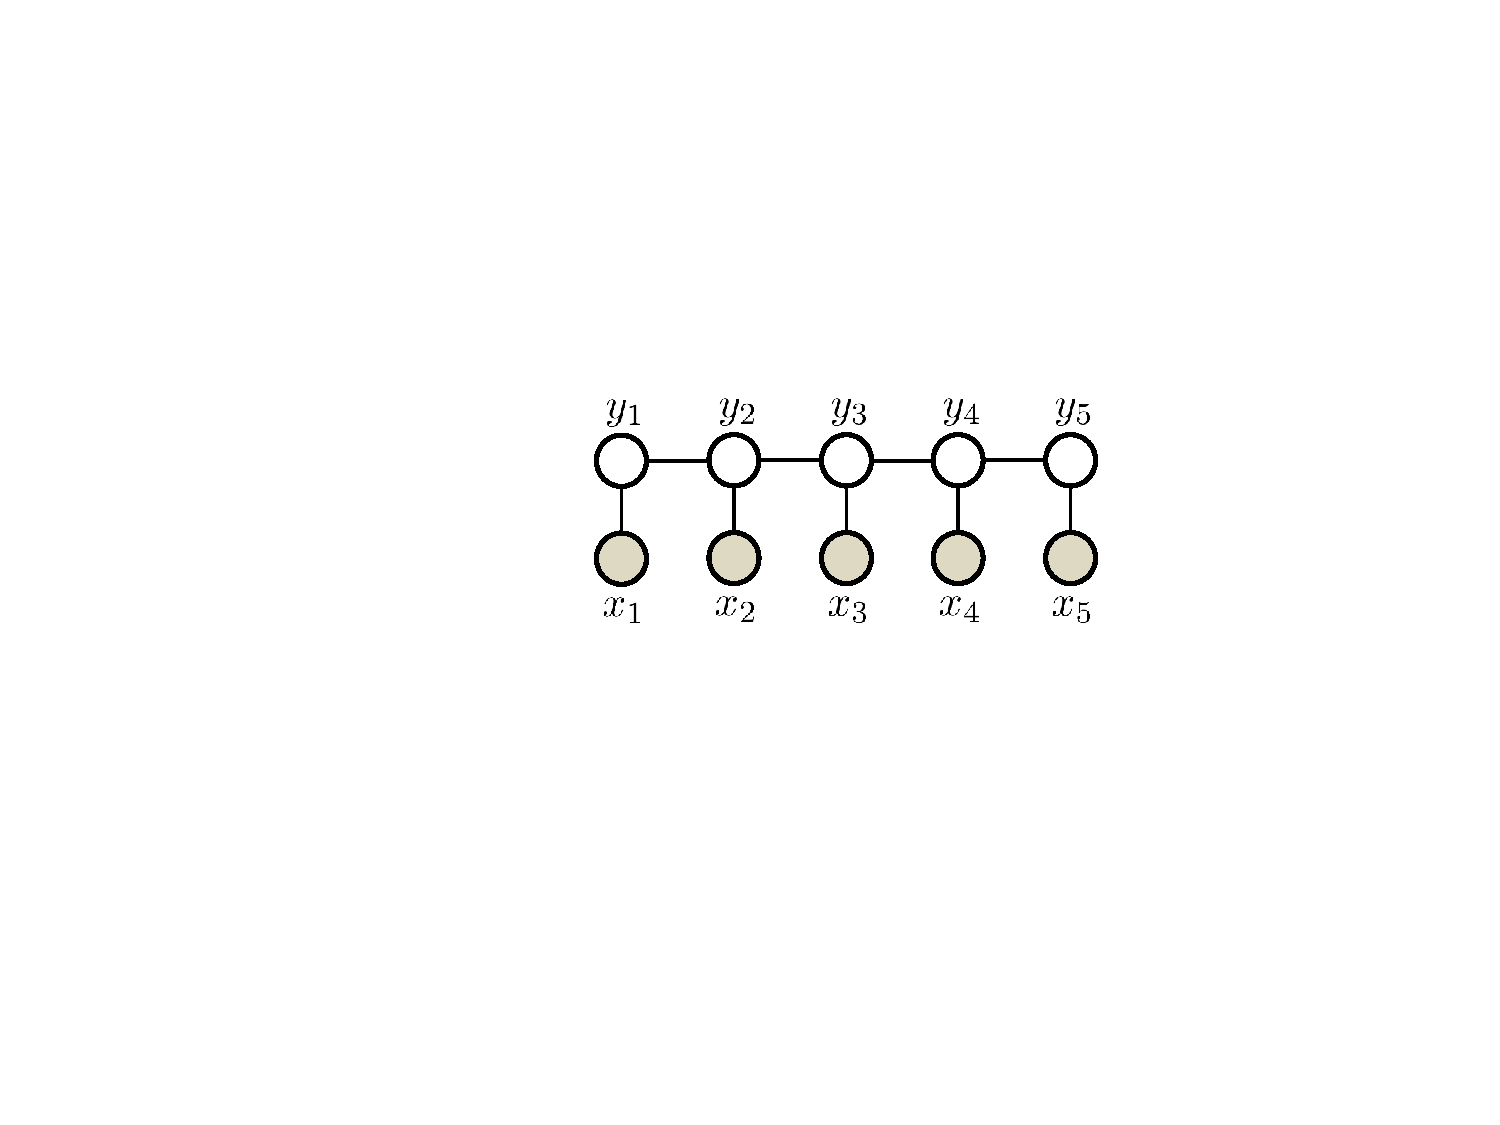
\includegraphics[width=5cm]{crf}
			\caption{CRF for word-letter}\label{fig:CRF_model}
		\end{minipage}
	\end{figure}
	
	
	
	\paragraph{Dataset}
	The original dataset was maintained by \href{https://en.wikipedia.org/wiki/Ben_Taskar}{Ben Taskar}.
	It contains the image and label of 6,877 words collected from 150 human subjects,
	with 52,152 letters in total.
	To simplify feature engineering, each letter image is encoded by a 128 (=16*8) dimensional vector,
	whose entries are either 0 (black) or 1 (white).
	%The code that loads the data always appends a constant 1 to the feature vectors,
	%leading to 129 features in total.
	The 6,877 words are divided evenly into training and test sets,
	provided in \verb#data/train.txt# and \verb#data/test.txt# respectively.
	The meaning of the fields in each line is described in \verb#data/fields_crf.txt#.
	
	
	Note in this dataset, only lowercase letters are involved, \ie\ 26 possible labels.
	Since the first letter of each word was capitalized and the rest were in lowercase,
	the dataset has removed all first letters.
	
	
	\paragraph{Performance measures}
	%
	We will compute two error rates: \emph{letter-wise} and \emph{word-wise}.
	Prediction/labeling is made on at letter level,
	and the percentage of incorrectly labeled letters is called letter-wise error.
	A word is correctly labeled if and only if \emph{all} letters in it are correctly labeled,
	and the word-wise error is the percentage of words in which at least one letter is mislabeled.
	
	
	\section{Conditional Random Fields}
	
	Suppose the training set consists of $n$ words.
	The image of the $t$-th word can be represented as
	$X^t = (\xvec^t_1, \ldots, \xvec^t_m)'$,
	where $'$ means transpose,
	$t$ is a superscript (not exponent),
	and each \emph{row} of $X^t$ (\eg\ $\xvec^t_m$) represents a letter.
	Here $m$ is the number of letters in the word,
	and $\xvec^t_j$ is a 128 dimensional vector that represents its $j$-th letter image.
	To ease notation, we simply assume all words have $m$ letters,
	and the model extends naturally to the general case where the length of word varies.
	The sequence label of a word is encoded as
	$\yvec^t = (y^t_1, \ldots, y^t_m)$,
	where $y^t_k \in \Ycal := \{1, 2, \ldots, 26\}$ represents the label of the $k$-th letter.
	So in Figure \ref{fig:brace}, $y^t_1 = 2$, $y^t_2 = 18$, \ldots, $y^t_5 = 5$.
	
	Using this notation, the Conditional Random Field (CRF) model for this task is a sequence shown in Figure \ref{fig:CRF_model},
	and the probabilistic model for a word/label pair $(X, \yvec)$ can be written as%
	\footnote{In statistics, random variables are generally written as capital letters.
		However using capital letters in the subscript really looks awkward, \eg, $\wvec_{Y_s}$,
		therefore we stick with lower case letter $\yvec$.}
	\begin{align}
		\label{eq:crf}
		p(\yvec | X ) &= \frac{1}{Z_X} \exp \rbr{\sum_{s=1}^m \inner{\wvec_{y_s}}{\xvec_s} + \sum_{s=1}^{m-1} T_{y_s, y_{s+1}}} \\
		\where Z_X &= \sum_{\hat{\yvec} \in \Ycal^m} \exp \rbr{\sum_{s=1}^m \inner{\wvec_{\yhat_s}}{\xvec_s} + \sum_{s=1}^{m-1} T_{\yhat_s, \yhat_{s+1}}}.
	\end{align}
	%
	%$Z(X)$ is a normalization constant depending on $X$.
	$\inner{\cdot}{\cdot}$ denotes inner product between vectors.
	Two groups of parameters are used here:
	
	\vspace{-1em}
	\begin{itemize}
		\item {\bf Node weight:} Letter-wise discriminant weight vector $\wvec_c \in \RR^{128}$ for each possible letter label $c \in \Ycal$.
		Note $c$ is different from $\yvec$,
		with the former being a letter label in $\Ycal$,
		while the latter being a \textit{sequence} of letter labels.
		%
		\item {\bf Edge weight:} Transition weight matrix $T$ which is sized $26$-by-$26$.
		$T_{ij}$ is the weight associated with the letter pair of the $i$-th and $j$-th letter in the alphabet.  For example $T_{1,9}$ is the weight for pair (`a', `i'), and $T_{24,2}$ is for the pair (`x', `b'). In general $T$ is not symmetric, \ie\ $T_{ij} \neq T_{ji}$, or written as $T' \neq T$ where $T'$ is the transpose of $T$.
	\end{itemize}
	
	Given these parameters (\eg\ by learning from data), the model \eqref{eq:crf} can be used to predict the sequence label (\ie\ word) for a new word image $X^* := (\xvec^*_1, \ldots, \xvec^*_m)^\top$ via the maximum a-posteriori (MAP) inference:
	\begin{align}
		\label{eq:crf_decode}
		\yvec^* = \argmax_{\yvec \in \Ycal^m} p(\yvec | X^*)
		= \argmax_{\yvec \in \Ycal^m} \cbr{ \sum_{s=1}^m \inner{\wvec_{y_s}}{\xvec^*_s} + \sum_{s=1}^{m-1} T_{y_s, y_{s+1}}}.
	\end{align}
	
	
	
	
	\begin{itemize}
		\item[(1a)] {\bf [5 Marks]} Show that for any $c \in \Ycal$, 
		$\grad_{\wvec_c} \log p(\yvec^t|X^t)$---the derivative of $\log p(\yvec^t|X^t)$ with respect to $\wvec_c$---can be written as:
		\begin{align}
			\grad_{\wvec_c} \log p(\yvec^t|X^t) & = \sum_{s=1}^m (\sembrack{y^t_s = c} - p(y_s = c | X^t)) \xvec^t_s,
		\end{align}
		where $\llbracket \cdot \rrbracket = 1$ if $\cdot$ is true, and 0 otherwise.
		Here $p(y_s | X^t)$ is the marginal distribution of $y_s$ given $X^t$ (based on \eqref{eq:crf}).
		Show your derivation step by step.
		
		Now derive the similar expression for $\grad_{T_{ij}} \log p(\yvec^t|X^t)$.
		
		\item[(1b)] {\bf [5 Marks]} A feature is a function that depends on $X$ and $\yvec$, but not $p(\yvec|X)$. Show that the gradient of $\log Z_X$ with respect to $\wvec_c$ and $T$ is exactly the expectation of some features with respect to $p(\yvec | X)$, and what are the features? Include your derivation.
		
		Hint: $T_{y_s, y_{s+1}} = \sum_{p \in \Ycal, q \in \Ycal} T_{pq} \cdot \llbracket (y_s, y_{s+1}) = (p,q)  \rrbracket$.
		
		\item[(1c)] 
		\label{qn:decoding}
		{\bf [12 Marks]} Implement the decoder \eqref{eq:crf_decode} with computational cost $O(m|\Ycal|^2)$.
		You may use the max-sum algorithm introduced in the course, or any simplified dynamic programming method that is customized to the simple sequence structure (see Appendix \ref{sec:MAP_formula}). 
		To keep it simple, you do not need to implement a full-fledged message passing algorithm.
		It is also fine to use the recursive functionality in the programming language.
		
		Also implement the brute-force solution by enumerating $\yvec \in \Ycal^m$, which costs $O(|\Ycal|^m)$ time.  Try small test cases to make sure your implementation of dynamic programming is correct.
		You may find \verb#itertools.product# useful.
		
		The project package includes a test case stored in \verb#data/decode_input.txt#.
		It has a single word with 100 letters ($\xvec_1, \ldots, \xvec_{100}$), $\wvec_c$, and $T$, stored as a column vector in the form of
		\begin{align}
			[\xvec'_1, \ldots, \xvec'_{100}, \wvec'_1, \ldots, \wvec'_{26}, T_{1,1}, T_{1,2}, \ldots, T_{1, 26}, T_{2,1}, \ldots, T_{2, 26}, \ldots, T_{26,1}, \ldots, T_{26, 26}]'.
		\end{align}
		All $\xvec_s \in \RR^{128}$ and $\wvec_c \in \RR^{128}$.
		
		\begin{center}
			\fbox{\begin{minipage}{38em}
					Be careful when loading $T$.  It is NOT a symmetric matrix.  
					Some languages store matrices in a \href{https://en.wikipedia.org/wiki/Row-_and_column-major_order}{row-major}
					order while some use column-major.
					So you need to decide whether the loaded $T$ needs to be transposed (I'm not hinting either way).
			\end{minipage}}
		\end{center}
		
		In your submission, create a folder \verb#result# and store the result of decoding (the optimal $\yvec^* \in \Ycal^{100}$ of \eqref{eq:crf_decode}) in \underline{\texttt{result/decode\_output.txt}}.
		It should have 100 lines,
		where the $i$-th line contains one integer in $\{1,\ldots,26\}$ representing $y^*_i$.
		In your report, provide the maximum objective value $\sum_{s=1}^m \inner{\wvec_{y_s}}{\xvec_s} + \sum_{s=1}^{m-1} T_{y_s, y_{s+1}}$ for this test case.
		If you are using your own dynamic programming algorithm (\ie\ not max-sum),
		give a brief description especially the formula of recursion.
	\end{itemize}
	
	%\newpage
	%Denote $m_{y_0 \to y_1}(y_1) = 1$ for all $y_1 \in \Ycal$.
	%
	%Forward: for $i = 2, 3, ... m-1$: $m_{y_i \to y_{i+1}}(y_{i+1}) = \sum_{y_i} m_{y_{i-1} \to y_{i}} (y_i)\exp (\inner{\wvec_{y_{i}}}{\xvec_i}) \exp(T_{y_i,y_{i+1}})$.
	%
	%Compute $Z = \sum_{y_m} m_{y_{m-1} \to y_m}(y_m) \exp (\inner{\wvec_{y_{m}}}{\xvec_m})$.
	%
	%Denote $m_{y_{m+1} \to y_m}(y_m) = 1$ for all $y_m \in \Ycal$.
	%
	%Backward: for $i = m, m-1,... 2$: $m_{y_i \to y_{i-1}}(y_{i-1}) = \sum_{y_i} m_{y_{i+1} \to y_{i}} (y_i)\exp (\inner{\wvec_{y_{i}}}{\xvec_i}) \exp(T_{y_{i-1},y_{i}})$.
	%
	%Compute marginals on $y_i$ for $i=1,\ldots,m$:
	%$p(y_i) \propto m_{y_{i-1} \to y_i}(y_i) m_{y_{i+1} \to y_i} (y_i) \exp (\inner{\wvec_{y_{i}}}{\xvec_i})$, followed by local normalization.
	%
	%Compute marginals on edges for $i=1,\ldots, m-1$:
	%$$p(y_i, y_{i+1}) \propto
	%m_{y_{i-1} \to y_i}(y_i) m_{y_{i+2} \to y_{i+1}} (y_{i+1})
	%\exp (\inner{\wvec_{y_{i}}}{\xvec_i})
	%\exp (\inner{\wvec_{y_{i+1}}}{\xvec_{i+1}})
	%\exp (T_{y_i, y_{i+1}}).$$
	%
	%Gradient in $\log Z$ are feature expectations computed from $p(y_i)$ and $p(y_i, y_{i+1})$.
	%\newpage
	
	\section{Training Conditional Random Fields}
	
	Finally, given a training set $\{X^t, \yvec^t\}_{t=1}^n$ ($n$ words),
	we can estimate the parameters $\{\wvec_c : c \in \Ycal\}$ and $T$ by maximizing the likelihood of the conditional distribution in \eqref{eq:crf}, or equivalently
	\begin{align}
		\label{eq:obj_MLE}
		\min_{\{\wvec_c\}, T} \ -\frac{C}{n}\sum_{t=1}^n \log p(\yvec^t | X^t) 
		+ \frac{1}{2} \sum_{c \in \Ycal} \nbr{\wvec_c}^2 
		+ \frac{1}{2} \sum_{ij} T^2_{ij}.
	\end{align}
	Here $C > 0$ is a trade-off weight that balances log-likelihood and regularization.
	
	
	\begin{itemize}
		\item[(2a)] {\bf [12 Marks]} Implement a dynamic programming algorithm to compute $\log p(\yvec^t | X^t)$ and its gradient.  Recall that the gradient is nothing but the expectation of features, and therefore it suffices to compute the marginal distribution of $y_j$ and $(y_s, y_{s+1})$. See Appendix \ref{sec:marginal}.
		The underlying dynamic programming principle is common to the computation of $\log p(\yvec^t | X^t)$, its gradient, and the decoder of \eqref{eq:crf_decode}.
		See Appendix \ref{sec:partition}.
		
		For numerical robustness (overflow or underflow), the following trick\footnote{\href{https://en.wikipedia.org/wiki/LogSumExp}{\url{https://en.wikipedia.org/wiki/LogSumExp}}} is widely used when computing $\log \sum_i \exp(x_i)$ for a given array $\{x_i\}$.  If we naively compute and store $\exp(x_i)$ as intermediate results, underflow and overflow could often occur.  So we resort to computing an equivalent form $M + \log \sum_i \exp(x_i - M)$, where $M := \max_i x_i$.  This way, the numbers to be exponentiated are always non-positive (eliminating overflow), and one of them is 0 (hence underflow is not an issue).  Similar tricks can be used for computing $\exp(x_1) / \sum_i \exp(x_i)$, or its logarithm.
		Do not use \verb#scipy.special.logsumexp#.
		
		For computational efficiency, pre-compute $\{\inner{\wvec_y}{\xvec_s}\}$ for all $y \in \Ycal$, $s \in \{1, \ldots, m\}$ before running the dynamic programming,
		so that they do not need to be recomputed in every step of the dynamic programming.
		
		To ensure your implementation is correct, it is recommended that the computed gradient be compared against the result of auto-differentiation (which is based only on the objective value).
		In Python, use \verb#scipy.optimize.check_grad#.	
		In general, it is a very good practice to use these tools to test the implementation of function evaluator.
		Since numerical differentiation is often computation intensive, you may want to design small test cases (\eg\ a single word with 4 letters, 4 randomly valued pixels, and 3 letters in the alphabet).
		An error level of $10^{-4}$ will be good enough.
		
		The project package includes a (big) test case in \verb#data/model.txt#.
		It specifies a value of $\wvec_c$ and $T$ as a column vector (again $T \neq T'$):
		\begin{align}
			\label{eq:model_vec}
			[\wvec'_1, \ldots, \wvec'_{26}, T_{1,1}, T_{1,2}, \ldots, T_{1, 26}, T_{2,1}, \ldots, T_{2, 26}, \ldots, T_{26,1}, \ldots, T_{26, 26}]'.
		\end{align}
		Compute the gradient $\frac{1}{n} \sum_{t=1}^n \grad_{\wvec_c} \log p(\yvec^t | X^t)$ and
		$\frac{1}{n} \sum_{t=1}^n \grad_{T} \log p(\yvec^t | X^t)$
		(\ie\ averaged over the training set provided in \verb#data/train.txt#) evaluated at this $\wvec_c$ and $T$.
		Store them in \underline{\texttt{result/gradient.txt}} as a column vector following the same order as in \eqref{eq:model_vec}.
		Pay good attention to column-major / row-major of your programming language when writing $T$.
		
		{\bf Provide} the value of $\frac{1}{n} \sum_{t=1}^n \log p(\yvec^t | X^t)$ for this case in your report.
		Hint: it is in $[-100,0]$.
		
		
		For your reference,
		in your instructor's Python implementation,
		it takes 5 seconds to compute the gradient on the whole training set.
		Single core of Intel(R) i7-10510U CPU @ 1.80GHz.
		
		
		\item[(2b)] {\bf [12 Marks]} We can now learn ($\{\wvec_c\}, T$) by solving the optimization problem in \eqref{eq:obj_MLE} based on the training examples in \verb#data/train.txt#.
		Set $C = 1000$.
		Typical off-the-shelf solvers rely on a routine which, given as input a feasible value of the optimization variables ($\wvec_c, T$), returns the objective value and gradient evaluated at that ($\wvec_c, T$). This routine is now ready from the above task,
		although you still need to compute the gradient of $\frac{1}{2} \sum_{c \in \Ycal} \nbr{\wvec_c}^2 + \frac{1}{2} \sum_{ij} T^2_{ij}$ in \eqref{eq:obj_MLE}.
		
		In this lab, we will use \href{https://docs.scipy.org/doc/scipy/reference/generated/scipy.optimize.fmin_tnc.html}{\texttt{fmin\_tnc}} (LBFGS) from \verb#scipy.optimize#, with the input argument \verb#bounds=none#.	
		Set the initial values of $\{\wvec_c\}$ and $T$ to zero.
		\href{https://www.programcreek.com/python/example/114546/scipy.optimize.fmin_tnc}{Here} are some examples of its use.
		
		Optimization solvers usually involve a large number of parameters.
		Some default settings for Python solvers are provided in \verb#code/ref_optimize.py#,
		where comments are included on the meaning of the parameters and other heuristics.
		It also includes some pseudo-code of CRF objective/gradient,
		to be used by various solvers.
		Feel free to tune the parameters of the solvers if you understand them.
		
		In your submission, include
		\begin{itemize}
			\item The optimal solution $\{\wvec_c\}$ and $T$.  Store them as \underline{\tt{result/solution.txt}}, in the format of \eqref{eq:model_vec}.
			%
			\item The predicted label for each letter in the test data \verb#data/test.txt#, using the decoder implemented in (1c).
			Store them in \underline{\tt{result/prediction.txt}},
			with each line having one integer in $\{1,\ldots, 26\}$ that represents the predicted label of a letter, in the same order as it appears in \verb#data/test.txt#.
		\end{itemize}
		In your report, provide the optimal objective value of \eqref{eq:obj_MLE} found by your solver.
	\end{itemize}
	
	
	\section{Benchmarking with Other Learning Models}
	
	In Question 2, we have managed to train the CRF,
	and the result can be used to make predictions on test sequences of images by running the decoding algorithm from Question 1c. 
	Now we can perform some benchmarking by comparing CRF with two alternative approaches:
	multi-class linear SVM on individual letters (SVM-MC),
	and structured SVM (SVM-Struct).
	SVM-MC treats each pair of \emph{letter} image and label as a training/test example.
	We will use the LibLinear package%
	\footnote{\href{http://www.csie.ntu.edu.tw/~cjlin/liblinear/}{http://www.csie.ntu.edu.tw/$\sim$cjlin/liblinear/}},
	which provides a Python wrapper.
	In order to keep the comparison fair,
	we will use linear kernels only (there are kernelized versions of CRF),
	and for linear kernels LibLinear is much faster than the general-purpose package LibSVM%
	\footnote{\href{http://www.csie.ntu.edu.tw/~cjlin/libsvm/}{http://www.csie.ntu.edu.tw/$\sim$cjlin/libsvm/}},
	
	
	For SVM-Struct, we will use the off-the-shelf implementation from the $\text{SVM}^{\text{hmm}}$ package%
	\footnote{\href{http://www.cs.cornell.edu/People/tj/svm_light/svm_hmm.html}{http://www.cs.cornell.edu/People/tj/svm\_light/svm\_hmm.html}},
	where some parameters are inherited from the $\text{SVM}^{\text{Struct}}$ package%
	\footnote{\href{http://www.cs.cornell.edu/people/tj/svm_light/svm_struct.html}{http://www.cs.cornell.edu/people/tj/svm\_light/svm\_struct.html}}.
	Do NOT use the $\text{SVM}^{\text{Struct}}$ package directly; 
	use the $\text{SVM}^{\text{hmm}}$ package instead.
	No Matlab/Python wrapper for $\text{SVM}^{\text{hmm}}$ is available.
	So write up a script in your favorite language to call the \textbf{binary} executables and to parse the results.
	
	
	$\text{SVM}^{\text{hmm}}$ requires that the input data be stored in a different format.
	This conversion has been done for you, and the resulting data files are \verb#data/train_struct.txt# and \verb#data/test_struct.txt#.
	For SVM-MC, you need to write a script to create a data file that is readable by LibSVM,
	and you may find it convenient to do it based on \verb#train_struct.txt# and \verb#test_struct.txt#.
	The meaning of the fields in each line is described in \verb#data/fields_struct.txt#.
	%Letter-wise multi-class SVM can be considered as a special case of structured SVM,
	%where each word consists of only one letter.
	
	
	
	
	\begin{itemize}
		\item[(3a)] {\bf [10 Marks]} $\text{SVM}^{\text{hmm}}$ has a number of parameters related to modeling, such as \verb#-c#, \verb#-p#, \verb#-o#, \verb#--t#, and \verb#--e#.
		Use the default settings for all parameters except \verb#-c#,
		which serves the same role as $C$ in \eqref{eq:obj_MLE} for CRF.
		In the sequel, we will also refer to the $C$ in \eqref{eq:obj_MLE} as the \verb#-c# parameter.
		LibLinear, which is used for SVM-MC, also has this parameter.
		But note that different from $\text{SVM}^{\text{hmm}}$ and \eqref{eq:obj_MLE}, the objective function used by LibLinear does NOT divide $C$ by the number of training examples (\ie\ letters).
		Keep the default value of other parameters in LibLinear.
		%So when invoking LibLinear, the value following \verb#-c# should be manually divided by $n$.
		
		The performance measure can be a) accuracy on letter-wise prediction, \ie\ the percentage of correctly predicted letters on the whole test set%
		\footnote{This is different from computing the percentage of correctly predicted letters in each word, and then averaging over all words, which is the last line of console output of \textsf{svm\_hmm\_classify}.  Both measures, of course, make sense.
			You may use the letter-wise prediction that \textsf{svm\_hmm\_classify} writes to the file specified by the third input argument.},
		or b) word-wise prediction, \ie\ the percentage of words whose constituent letters are all predicted correctly.
		For multi-class problems, accuracy is more commonly used than error.
		
		For each of CRF, SVM-Struct, and SVM-MC,
		plot a curve in a separate figure where the $y$-axis is the letter-wise prediction accuracy on test data,
		and the $x$-axis is the value of \verb#-c# varied in a range that you find reasonable,
		\eg\ $\{1, 10, 100, 1000\}$.
		Theoretically, a small \verb#-c# value will ignore the training data and generalize poorly on test data.
		On the other hand, overly large \verb#-c# may lead to overfitting, and make optimization challenging (taking a lot of time to converge).
		
		\textbf{Hint}: to roughly find a reasonable range of \verb#-c#, a commonly used heuristic is to try on a small sub-sample of the data, and then apply it to a larger data set (be wary of normalization by the number of training example for LibLinear as mentioned above).
		
		What observation can be made on the result?
		
		\item[(3b)] {\bf [5 Marks]} Produce another three plots for word-wise prediction accuracy on test data.  What observation can be made on the result?
		%Note in SVM-MC, we used the trick of treating each letter as a word. Therefore some conversion is needed to compute the word-wise accuracy. So another file \verb#data/test_index.txt# is provided.  Each line of it corresponds to a letter in the test set, and it has the same number of lines as \verb#test_mc.txt#.  Each line has a single integer which is the word-id from the original data.  So two lines with the same integer means their corresponding letters belong to the same word.
	\end{itemize}
	
	
	\section{Stochastic Optimization}
	
	\begin{figure}[t]
		\centering
		\subfigure[Training objective v.s. effective pass]{
			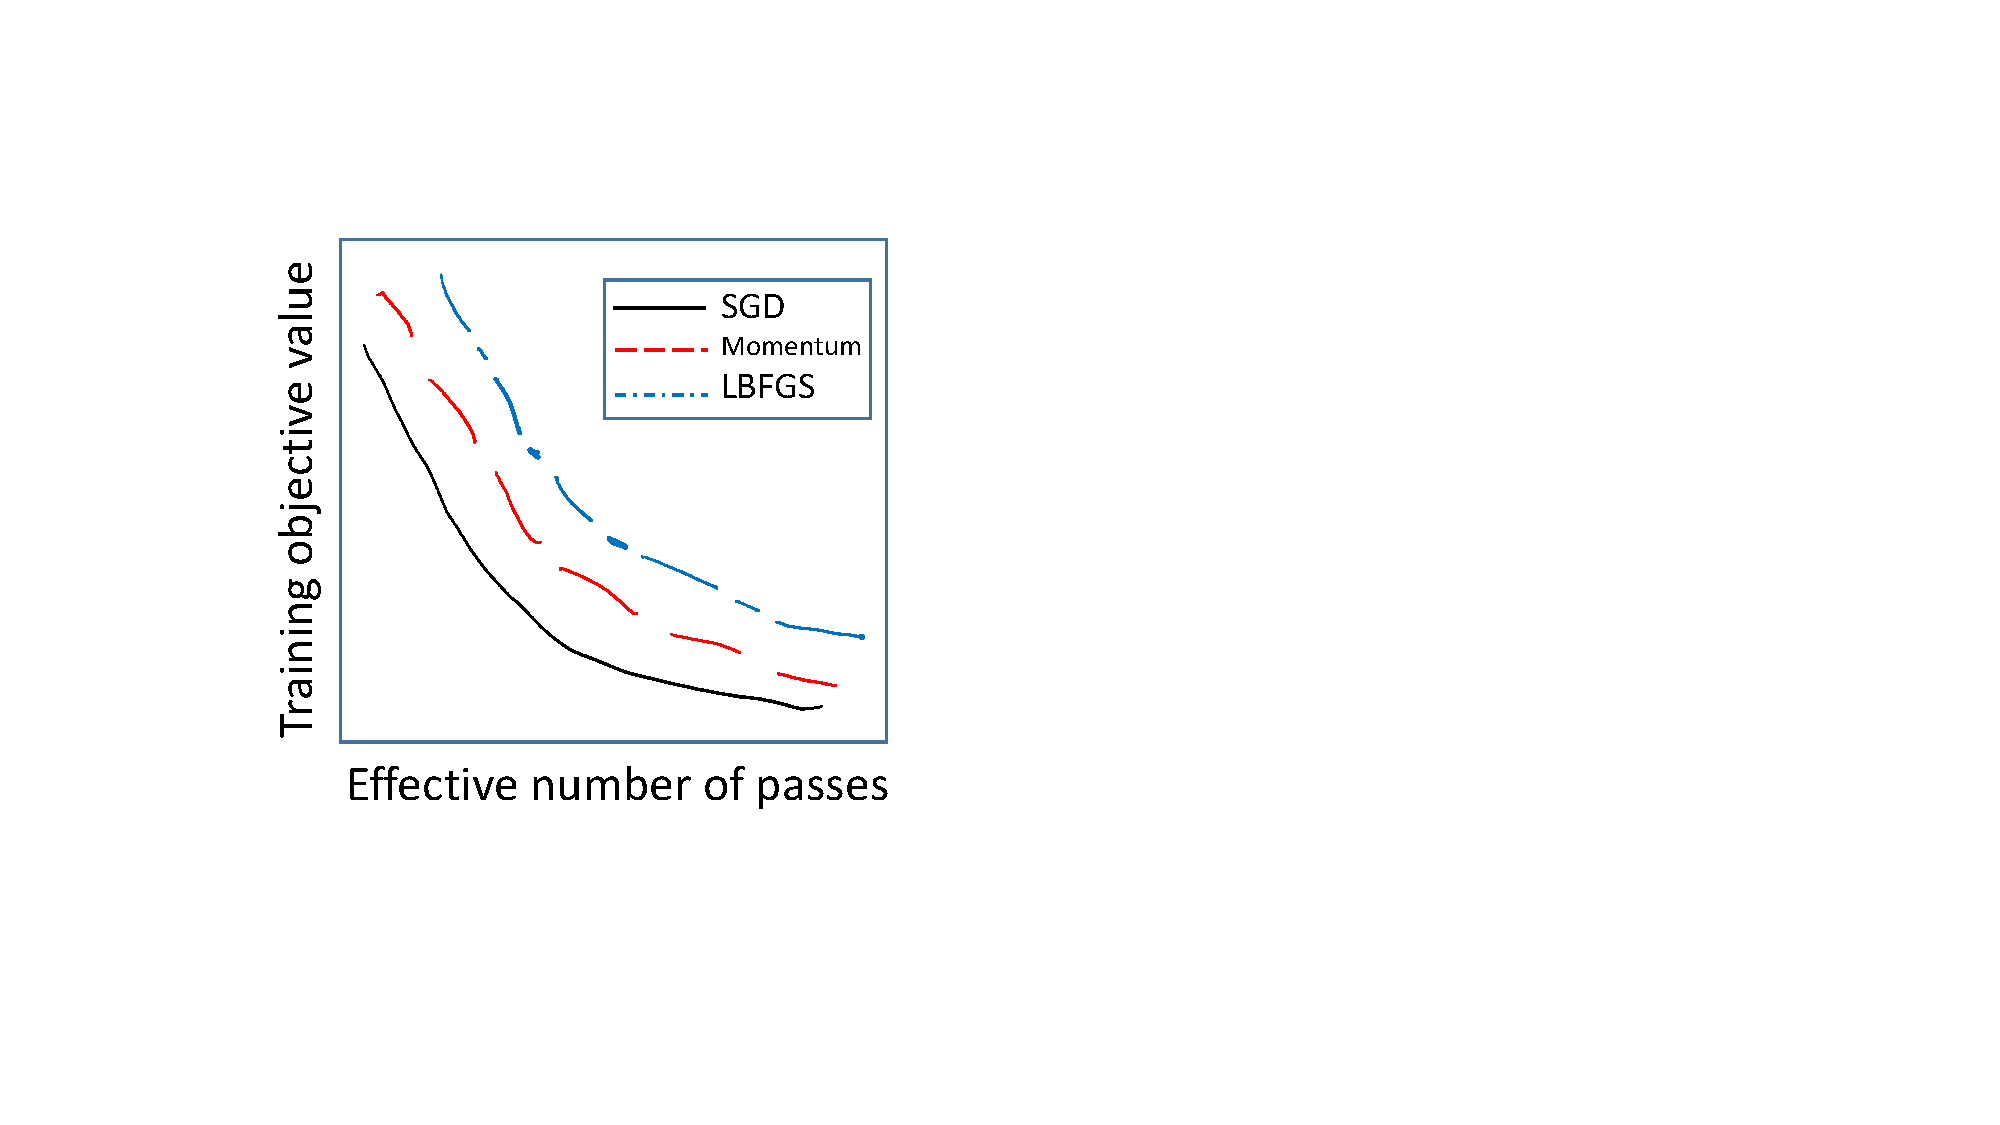
\includegraphics[width=6cm]{obj_compare}}
		\hspace{4em}
		\subfigure[Test word-wise error v.s. effective pass]{
			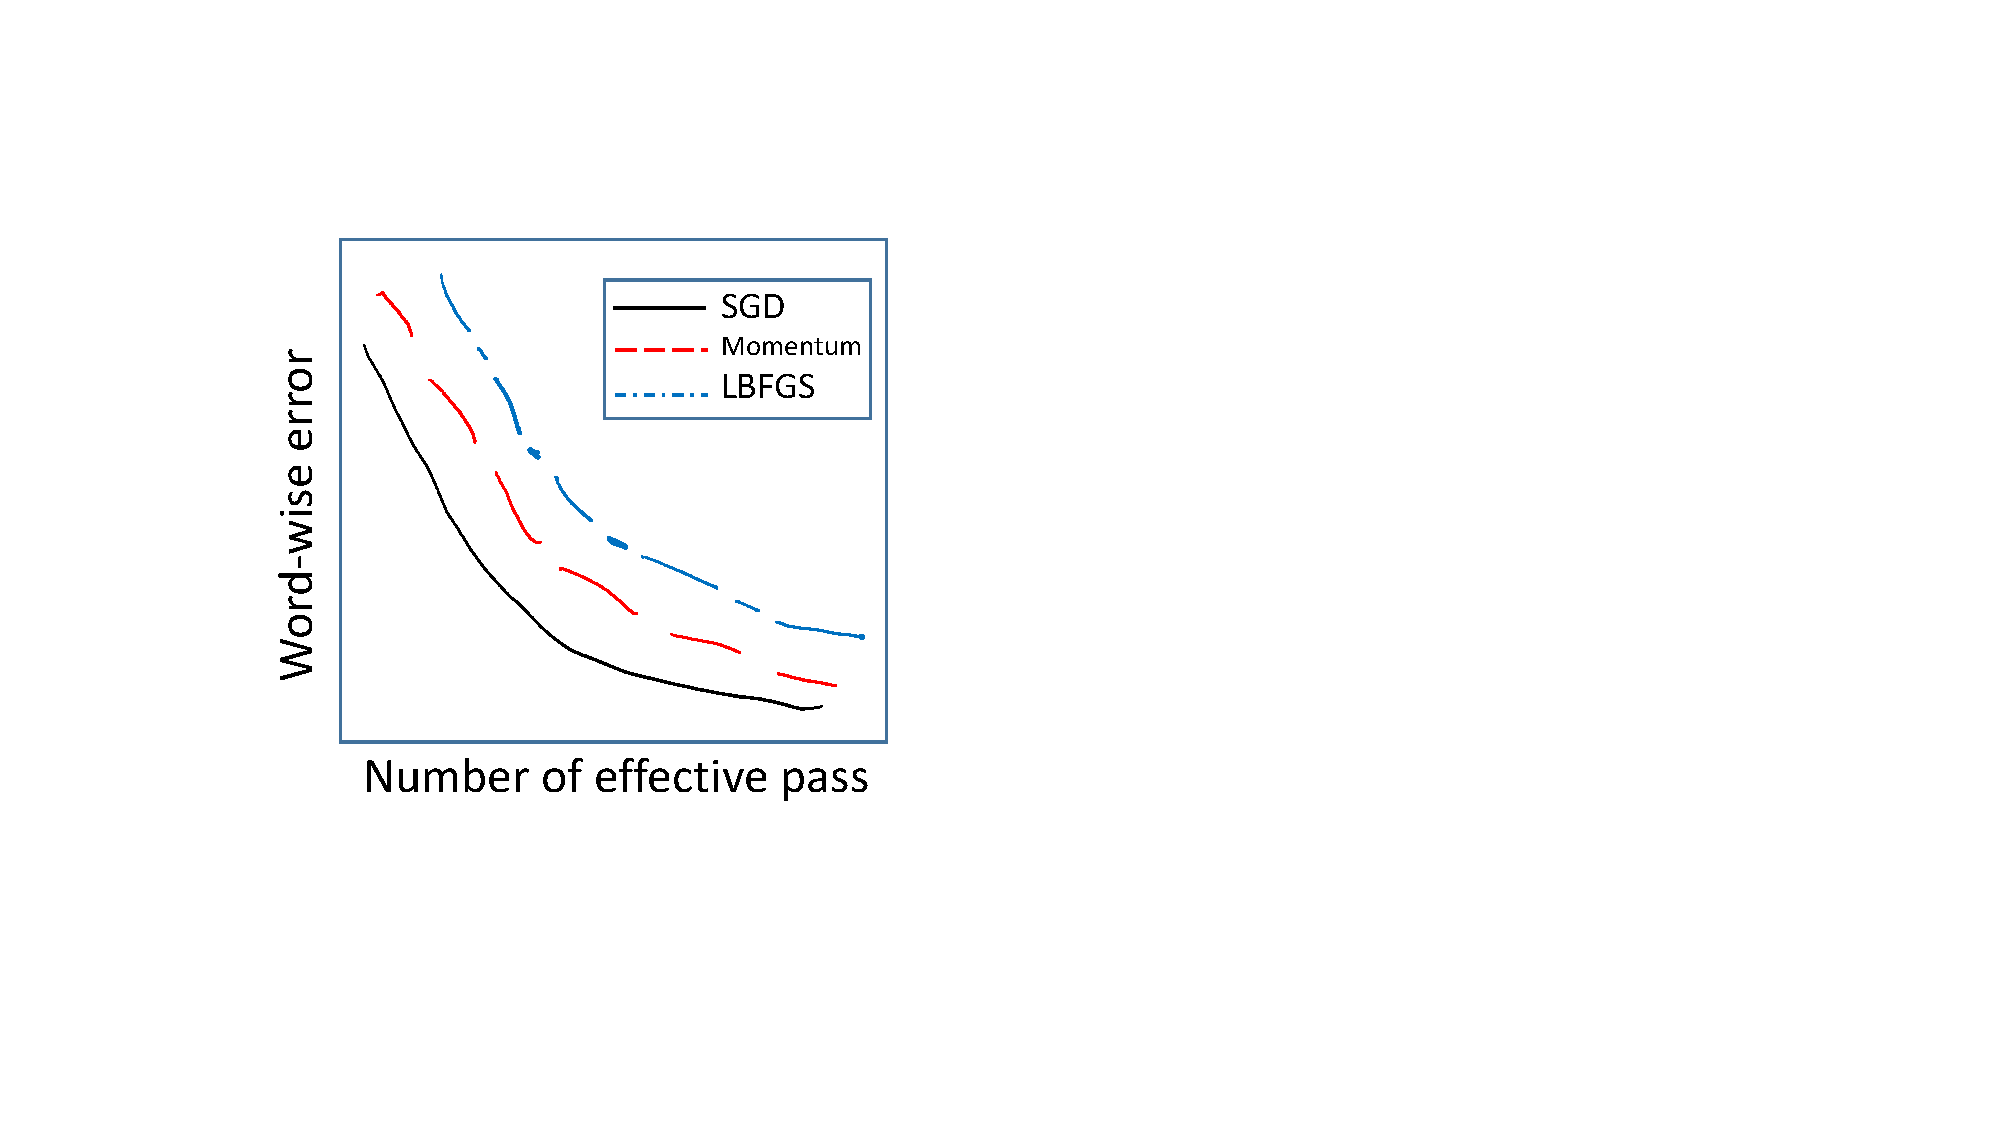
\includegraphics[width=6cm]{error_compare}}
		\caption{Comparison of SGD, momentum, and LBFGS}
		\label{fig:compare_optimizer}
	\end{figure}
	
	
	So far, we have trained CRF (\ie, solving \eqref{eq:obj_MLE}) by batch optimization.
	We now test stochastic optimization in two senses:
	stochastic mini-batch and sampling based inference.
	For this section, you should fix the value of $C$ in the CRF to the best value found by the previous section.
	%
	\begin{itemize}
		\item[(4a)] {\bf [8 Marks]}
		The idea of stochastic optimization is very simple. 
		At each iteration, we randomly sample $B$ number of training examples (denoted as $\Bcal$), 
		and approximate $\frac{1}{n}\sum_{t=1}^n \log p(\yvec^t | X^t)$
		by $\frac{1}{B}\sum_{t\in \Bcal} \log p(\yvec^t | X^t)$.
		Using the (stochastic) gradient computed from the latter, 
		we can run multiple solvers such as stochastic gradient descent (SGD)
		and SGD with momentum.
		Read the following \href{https://machinelearningmastery.com/gradient-descent-with-momentum-from-scratch/}{blog} and import its implementation of the two algorithms to your project.
		
		
		Our goal is to compare the efficiency of SGD, momentum, and LBFGS in driving down the training objective \eqref{eq:obj_MLE} and in reducing the test error.
		To this end, we will plot two figures, each including three curves corresponding to the  three methods (see an example plot in Figure \ref{fig:compare_optimizer}).
		The first figure illustrates the decline of training objective value (\ie, \eqref{eq:obj_MLE}) as a function of effective number of passes.
		Suppose SGD is run for $k$ iterations/steps, with each iteration sampling $B$ examples/words.
		Then the effective number of pass is $kB/n$,
		facilitating the comparison with LBFGS,
		where the effective number of pass is exactly the number of objective function evaluation.
		It is crucial to note that each iteration of LBFGS may evaluate the function \textbf{more than once}.
		\verb#fmin_tnc# takes a callback function, which will help us to track the progress.
		However, the callback function only takes as input the current solution,
		and does not provide the count of function evaluation so far.
		As a hack, you can put a counter in the function evaluation subroutine written by yourself,
		and make it a global variable which can be accessed inside the callback function.
		
		Within the callback function, evaluate and print two numbers: 
		1) the word-wise test error given by the current value of $\{w_c\}$ and $T$;
		2) the current training objective value of \eqref{eq:obj_MLE}.
		For the latter, simply (re)compute the objective value instead of buffering the value from the last function evaluation; the mechanism of LBFGS may mess it up.
		You can also save the values of 1) and 2) as global variables,
		which can be used for plotting after the solver terminates.
		
		All the three solvers have hyperparameters, including $B$ and learning rate for SGD and momentum.
		Tune them well for all the methods respectively before plotting.
		You can tune them based on how fast the training objective decays.
		%
		\item[(4b)] {\bf [8 Marks]} 
		Since the dynamic programming based gradient computation can still be expensive,
		an alternative is to evaluate the gradient by sampling,
		noting that the gradient only requires the marginal distribution on edges and nodes.
		Here, let us use a block Markov Chain Monte Carlo (MCMC) sampler,
		which is the method of training restricted Boltzmann machines:	
		
		1. Ignore the edge potential (\ie, set $T=\zero$), which leaves all $y_s$ as independent given $X$.
		
		2. Sample the value of $y_s$ for all $s$ based on such independent distributions.
		
		3. For $k = 1, 2, \ldots, S$ ($S$ being a hyperparameter for tuning, akin to $B$)
		
		4. $\qquad$ Given/fixing $y_1, y_3, y_5, \ldots$, sample for $y_2, y_4, y_6, \ldots$ ($T$ is no longer set to $\zero$).
		
		5. $\qquad$ Given/fixing $y_2, y_4, y_6, \ldots$, sample for $y_1, y_3, y_5, \ldots$ ($T$ is no longer set to $\zero$).
		
		6. $\qquad$ Call the current $\{y_1, y_2, y_3, y_4, \ldots\}$ as a \textbf{sample}.
		
		7. Use the $S$ samples to compute the marginal distribution of nodes and edges.
		
		The key convenience is that given $y_1, y_3, y_5, \ldots$, 
		the remaining variables $y_2, y_4, y_6, \ldots$ are independent, hence can be sampled independently and efficiently.
		Overall we draw $S$ number of samples.
		
		
		
		
		Answer the following questions in your report.
		
		\textbf{(i)} 
		Write out the formula of $p(y_s|\ldots, y_{s-3}, y_{s-1}, y_{s+1}, y_{s+3}, \ldots, X)$.
		There is no need to distinguish odd or even values of $s$. 
		What is the overall computational complexity (in big $O$ notation) of drawing a sample, \ie, completing steps 4 and 5 for one iteration of $k$.
		Compare it with the cost of dynamic programming.
		Your complexity should be expressed in the number of letters in the word ($m$),
		and the size of the alphabet (\ie, $\abr{\Ycal}=26$).
		
		Incidentally, you may have noticed that it is even more time consuming to draw a reasonable number of samples than to run the dynamic programming.
		This is expected because we are working on a linear chain on which dynamic programming is feasible.
		But sampling can be applied to a far broader range of graphs,
		and our focus in this lab is to explore how many samples are needed to get a good gradient.
		
		\textbf{(ii)} 
		Implement the sampling procedure and supply the resulting gradient to SGD, momentum, LBFGS.
		In a sense, it is doubly stochastic for SGD and momentum, because both the mini-batch and MCMC introduce noise. 
		In contrast, the gradient used by LBFGS is noisy only due to MCMC,
		and it still uses the entire training set.
		Now reproduce the two plots in the same way as in Question 4a.
		
		
		What observations can you make?  How does $S$ impact the performance of the three solvers?
		You can directly reuse the best hyperparameters of the three solvers from Question 4a.
		
		\textbf{Hint}: You do not need to use a large number of samples.  $S=10$ or even 5 might work.
		
		\textbf{How to debug your sampler?} The easiest way is to take an arbitrary word, and compute the node and edge marginal distributions based on samples.  Then compare them with the result of dynamic programming.  The difference should decay to 0 as $S$ grows.
		
		\item[(4c)] {\bf [8 Marks]} 
		Rao-Blackwellization. 
		MCMC can require a lot of samples if we really want high-quality estimates of node and edge distributions.
		It may also suffer from high variance.
		To alleviate this problem, the Rao-Blackwell approach is handy.
		Instead of counting hard samples (0/1), it accumulates fractional samples.
		For example, previously, when a sample 'a' is drawn for $y_k$, 
		we just increment the count of $y_k = $'a' by 1 for the purpose of estimating the marginal probability of $y_k$.
		Now suppose $p=(p_a, \ldots, p_z)$ is the conditional probability of $y_k$ given $y_1, \ldots, y_{k-1}, y_{k+1}, \ldots$ (step 4 or 5 in the above algorithm), then we will increment the count of $y_k = $'a' by $p_a$,
		the count of $y_k = $'b' by $p_b$, etc.
		
		Similar ideas can be extended to edge marginals.
		Suppose, when we draw sample for $y_k$, 
		the current sampled letter value of $y_{k-1}$ and $y_{k+1}$ is 'r' and 's', respectively.
		Then we will increment the count for $P_{k-1,k}(r, a)$ by $p_a$, 
		the count for $P_{k-1,k}(r, b)$ by $p_b$, 
		the count for $P_{k,k+1}(a, s)$ by $p_a$, 
		the count for $P_{k,k+1}(b, s)$ by $p_b$, 
		etc.
		Here $P_{k-1,k}$ is the marginal distribution of $(y_{k-1}, y_k)$,
		and $P_{k,k+1}$ is the marginal distribution of $(y_k, y_{k+1})$.
		
		Now do the following in the report.
		
		\textbf{(i)}  Write out the pseudo-code for Rao-Blackwellized MCMC sampling.  
		You may doubt when to update the count:
		after sampling the entire sequence (as in the above algorithm),
		or right after each $y_k$ is drawn.
		You may also consider how to do the normalization.
		Use your own intuition and resort to experiment to figure out a reasonable algorithm.
		The `correct' algorithm is not unique, and it works when the divergence against the dynamic programming result decays to 0 as more and more samples are drawn.
		See the next sub-question (ii).
		
		\textbf{(ii)} Take the model in \verb#data/model.txt# and the first word in \verb#data/train.txt#. Then plot in one figure the KL-divergence between MCMC estimate $\ptil$ and the dynamic programming result $p$, with or without Rao-Blackwellization.
		The x-axis is the number of samples,
		and the y-axis is 
		$\sum_{s=1}^m \text{KL}(\ptil_s, p_s)$ (for node marginal) and 
		$\sum_{s=1}^{m-1} \text{KL}(\ptil_{s,s+1}, p_{s,s+1})$ (for edge marginal).
		Multiplied with using and not using Rao-Blackwellization,
		there should be \textbf{four} curves in the plot.
		If it helps, use logarithmic scale for some axis.
		What observation can be made?
	\end{itemize}
	
	
	
	
	\section{Robustness to Distortion}
	
	An evil machine learner tampered with the training and test images by rotation and translation.
	However, the labels (letter/word annotation) are still clean, and so
	one could envisage that the structured models (CRF and SVM-Struct) will be less susceptible to such tempering.
	
	
	
	In Python, you can use functions from OpenCV such as
	\href{https://docs.opencv.org/3.4/da/d54/group__imgproc__transform.html#gafbbc470ce83812914a70abfb604f4326}{\texttt{getRotationMatrix2D}} and \href{https://docs.opencv.org/3.4/da/d54/group__imgproc__transform.html#ga0203d9ee5fcd28d40dbc4a1ea4451983}{\texttt{warpAffine}} to rotate and translate an image. 
	They take some parameters such as offset and degree of rotation.
	Make sure that the image size is not changed. 
	This means in \texttt{warpAffine}, set the argument \verb#dsize# appropriately.
	You can choose any interpolation method.
	%
	Both functions take images represented as a matrix.
	So if your image is represented as a 128 dimensional vector,
	first reshape it into a matrix sized $8 \times 16$,
	then apply these functions,
	followed by vectorizing it back.
	
	The images stored in the data files are in \href{https://en.wikipedia.org/wiki/Row-_and_column-major_order}{column-major order}.
	In contrast, Python uses row-major.
	As you need to translate and rotate images here, 
	you may want to ensure that the 2-D image is properly loaded before applying the transformations.  
	Just check by visualizing the images, e.g. by \verb#imshow#.	
	
	In this experiment
	we randomly select a subset of training examples to distort.
	All test examples remain unchanged.
	A randomly generated list of transformations are given in \verb#data/transform.txt#, where the lines are in the following format:
	%
	\begin{verbatim}
		r 317 15
		t 2149 3 3
	\end{verbatim}
	The first line means: on the 317-th word of the training data (in the order of \verb#train.txt#),
	apply counterclockwise rotation by 15 degrees \emph{to all its letters}.
	The second line means on the 2149-th word of the training data, apply translation with offset $(3,3)$.
	Note in each line the first number (\ie\ second column: 317, 2149, \ldots) is random and \emph{not} sorted.
	All line numbers appear exactly once.
	
	\begin{itemize}
		\item[(5a)] {\bf [10 Marks]} In one figure, plot the following two curves where the $y$-axis is the letter-wise prediction accuracy on test data.  We will apply to the training data the first $x$ lines of transformations specified in \verb#data/transform.txt#.  $x$ is varied in $\{0, 500, 1000, 1500, 2000\}$ and serves as the value of $x$-axis.
		
		1) CRF where the \verb#-c# parameter is set to any of the best values found in (3a);
		
		2) SVM-MC where the \verb#-c# parameter is set to any of the best values found in (3a).
		
		What observation can be made on the result?
		
		\item[(5b)] {\bf [5 Marks]}  Generate another plot for word-wise prediction accuracy on test data.  The \verb#-c# parameter in SVM-MC may adopt any of the best values found in (3b).
		What observation can be made on the result?
		
	\end{itemize}
	
	\newpage
	\section{Appendix: Dynamic programming details}
	
	\subsection{Computing the partition function}
	\label{sec:partition}
	
	In order to compute $Z$, let us define $f_1(y_1) = 1$ for all $y_1 \in \Ycal$, and then for all $i = 2, \ldots, m$
	\begin{align}
		f_i(y_i) = \sum_{y_1, \ldots, y_{i-1}} \exp \rbr{\sum_{j=1}^{i-1} \inner{\wvec_{y_j}}{\xvec_j} + \sum_{j=1}^{i-1} T_{y_j, y_{j+1}}}, \quad \forall y_i \in \Ycal.
	\end{align}
	%This is exactly the message $m_{(i-1) \to i}(y_{i})$ defined in our lecture of Mar 1.
	Then
	\begin{align}
		Z = \sum_{y_m \in \Ycal} \exp \rbr{\inner{\wvec_{y_m}}{\xvec_m}} f_m(y_m) .
	\end{align}
	
	To compute $f_i(y_i)$, we use recursion by
	\begin{align}
		\label{eq:rec_Z_forward_1}
		f_1(y_1) &= 1, \quad \forall y_1 \in \Ycal \\
		f_i(y_i) &= \sum_{y_{i-1}} \exp \rbr{\inner{\wvec_{y_{i-1}}}{\xvec_{i-1}} + T_{y_{i-1}, y_i}}
		\sum_{y_1, \ldots, y_{i-2}} \exp \rbr{\sum_{j=1}^{i-2} \inner{\wvec_{y_j}}{\xvec_j} + \sum_{j=1}^{i-2} T_{y_j, y_{j+1}}} \\
		\label{eq:rec_Z_forward_2}
		&= \sum_{y_{i-1}} \exp \rbr{\inner{\wvec_{y_{i-1}}}{\xvec_{i-1}} + T_{y_{i-1}, y_i}}  \cdot f_{i-1}(y_{i-1})  \qquad (\forall\ y_i \in \Ycal, \ i = 2, 3, \ldots, m).	 
	\end{align}
	
	\paragraph{Comment 1:}
	We can also use the log-sum-exp trick if we stay in the logarithmic space. 
	Define $\alpha_i(y_i) = \log f_i(y_i)$.
	Then $\alpha_1(y_1) = 0$, and
	\begin{align}
		\alpha_i(y_i) &= \log \sum_{y_{i-1}} \exp \rbr{\inner{\wvec_{y_{i-1}}}{\xvec_{i-1}} + T_{y_{i-1}, y_i} + \alpha_{i-1}(y_{i-1})} \qquad \forall i \ge 2, y_i \in \Ycal\\
		\log Z &= \log \sum_{y_m} \exp (\inner{\wvec_{y_m}}{\xvec_m} + \alpha_m(y_m)).
	\end{align}
	
	\paragraph{Comment 2:}
	We might attempt to incorporate the node factor $\exp(\inner{\wvec_{y_i}}{\xvec_i})$ into the message, i.e.,
	\begin{align}
		g_i(y_i) := \exp(\inner{\wvec_{y_i}}{\xvec_i}) \cdot f_i(y_i) = \sum_{y_1, \ldots, y_{i-1}} \exp \rbr{\sum_{j=1}^{i} \inner{\wvec_{y_j}}{\xvec_j} + \sum_{j=1}^{i-1} T_{y_j, y_{j+1}}}, \quad \forall y_i \in \Ycal.
	\end{align}
	Then the recursion can be written as
	\begin{align}
		g_1(y_1) &= \exp(\inner{\wvec_{y_1}}{\xvec_1}), \quad \forall y_1 \in \Ycal \\
		g_i(y_i) &= \exp(\inner{\wvec_{y_i}}{\xvec_i}) \cdot \sum_{y_{i-1}} \exp \rbr{T_{y_{i-1}, y_i}}
		\sum_{y_1, \ldots, y_{i-2}} \exp \rbr{\sum_{j=1}^{i-1} \inner{\wvec_{y_j}}{\xvec_j} + \sum_{j=1}^{i-2} T_{y_j, y_{j+1}}} \\
		&= \exp(\inner{\wvec_{y_i}}{\xvec_i}) \cdot \sum_{y_{i-1}} \exp \rbr{T_{y_{i-1}, y_i}}  g_{i-1}(y_{i-1})  \qquad (\forall\ i \ge 2, \ y_i \in \Ycal), \\
		\text{and} \quad Z &= \sum_{y_m} f_m(y_m).
	\end{align}
	This works well for a linear chain.
	But it is not recommended because it does not extend well to general tree structure.
	Suppose we want to compute the message from $j$ to $i$, and $j$ has two other neighbors $k$ and $k'$.
	Then the messages $k \to j$ and $k' \to j$ have \textbf{both} contained the node potential of $j$ (i.e. $f_j(y_j) = \exp (\inner{\wvec_{y_j}}{\xvec_j})$).
	So when we multiply together the messages $k \to j$ and $k' \to j$ (as in the message formula),
	this node potential will be \emph{double counted}.
	
	\subsection{MAP inference}
	\label{sec:MAP_formula}
	Here we define
	\begin{align}
		h_i(y_i) = \max_{y_1, \ldots, y_{i-1}} \exp \rbr{\sum_{j=1}^{i-1} \inner{\wvec_{y_j}}{\xvec_j} + \sum_{j=1}^{i-1} T_{y_j, y_{j+1}}}, \quad \forall y_i \in \Ycal.
	\end{align}
	
	Then all the recursion expressions in \eqref{eq:rec_Z_forward_1}	to \eqref{eq:rec_Z_forward_2} almost remain unchanged,
	except that all summations are replaced by max:
	\begin{align}
		\label{eq:rec_MAP_forward_1}
		h_1(y_1) &= 1, \quad \forall y_1 \in \Ycal \\
		h_i(y_i) &= \max_{y_{i-1}} \exp \rbr{\inner{\wvec_{y_{i-1}}}{\xvec_{i-1}} + T_{y_{i-1}, y_i}}
		\max_{y_1, \ldots, y_{i-2}} \exp \rbr{\sum_{j=1}^{i-2} \inner{\wvec_{y_j}}{\xvec_j} + \sum_{j=1}^{i-2} T_{y_j, y_{j+1}}} \\
		\label{eq:rec_MAP_forward_2}	
		&= \max_{y_{i-1}} \exp \rbr{\inner{\wvec_{y_{i-1}}}{\xvec_{i-1}} + T_{y_{i-1}, y_i}}  h_{i-1}(y_{i-1})  \qquad (\forall\ y_i \in \Ycal, \ i = 2, 3, \ldots, m).
	\end{align}
	
	After obtaining $h_m(y_m)$, we recover the MAP by backtracking
	\begin{align}
		y^*_m &= \argmax_{y_m} \cbr{ \exp(\inner{\wvec_{y_m}}{\xvec_m}) h_m(y_m)} \\
		y^*_{i-1} &= \argmax_{y_{i-1}} \exp \rbr{\inner{\wvec_{y_{i-1}}}{\xvec_{i-1}} + T_{y_{i-1}, y^*_i}}  h_{i-1}(y_{i-1})  \qquad (\forall\ i = m, m-1, \ldots, 2).
	\end{align}
	
	\paragraph{Comment 3:}
	The above algorithm is called max-product.
	We can also take the log of $h_i(y_i)$ and get the max-sum algorithm:
	\begin{align}
		l_i(y_i) = \log h_i(y_i) = \max_{y_1, \ldots, y_{i-1}} \cbr{\sum_{j=1}^{i-1} \inner{\wvec_{y_j}}{\xvec_j} + \sum_{j=1}^{i-1} T_{y_j, y_{j+1}}}.
	\end{align}
	
	And the recursion goes by
	\begin{align}
		l_1(y_1) &= 0, \quad \forall y_1 \in \Ycal \\
		l_i(y_i) &= \max_{y_{i-1}} \cbr{\inner{\wvec_{y_{i-1}}}{\xvec_{i-1}} + T_{y_{i-1}, y_i} + l_{i-1}(y_{i-1})}, \quad \forall y_i \in \Ycal.
	\end{align}
	And the recovery is
	\begin{align}
		y^*_m &= \argmax_{y_m} \cbr{ \inner{\wvec_{y_m}}{\xvec_m} + l_m(y_m)} \\
		y^*_{i-1} &= \argmax_{y_{i-1}} \cbr{ \inner{\wvec_{y_{i-1}}}{\xvec_{i-1}} + T_{y_{i-1}, y^*_i} + l_{i-1}(y_{i-1})}  \qquad (\forall\ i = m, m-1, \ldots, 2).
	\end{align}
	
	\subsection{Marginal distribution}
	\label{sec:marginal}
	
	To compute the marginal distribution, we need the backward messages.
	Define $b_m(y_m) = 1$ for all $y_m \in \Ycal$ and then for all $i = m-1, \ldots, 1$
	\begin{align}
		b_i(y_i) = \sum_{y_{i+1}, \ldots, y_{m}} \exp \rbr{\sum_{j=i+1}^m \inner{\wvec_{y_j}}{\xvec_j} + \sum_{j=i}^{m-1} T_{y_j, y_{j+1}}}, \quad \forall y_i \in \Ycal.
	\end{align}
	This is exactly the message $m_{(i+1) \to i} (y_i)$ defined in our lecture.
	Then the partition function can be computed by
	\begin{align}
		Z = \sum_{y_1} \exp \rbr{\inner{\wvec_{y_1}}{\xvec_1}} b_1(y_1).
	\end{align}
	
	
	To compute $b_i(y_i)$, we use recursion by
	\begin{align}
		\label{eq:rec_Z_forward_1}
		b_m(y_m) &= 1, \quad \forall y_i \in \Ycal \\
		b_i(y_i) &= \sum_{y_{i+1}} \exp \rbr{\inner{\wvec_{y_{i+1}}}{\xvec_{i+1}} + T_{y_{i}, y_{i+1}}}
		\sum_{y_{i+2}, \ldots, y_m} \exp \rbr{\sum_{j=i+2}^{m} \inner{\wvec_{y_j}}{\xvec_j} + \sum_{j=i+1}^{m-1} T_{y_j, y_{j+1}}} \\
		\label{eq:rec_Z_forward_2}
		&= \sum_{y_{i+1}}\exp \rbr{\inner{\wvec_{y_{i+1}}}{\xvec_{i+1}} + T_{y_{i}, y_{i+1}}} b_{i+1}(y_{i+1})  \qquad (\forall\ y_i \in \Ycal, \ i = m-1, m-2, \ldots, 1).	 
	\end{align}
	
	Finally, the marginal distribution of $y_i$ is
	\begin{align}
		p(y_i) \propto f_i(y_i) \cdot b_i(y_i) \cdot \exp \rbr{\inner{\wvec_{y_{i}}}{\xvec_{i}}},
	\end{align}
	followed by local normalization.
	Furthermore, the marginal distribution of $(y_i, y_{i+1})$ is
	\begin{align}
		p(y_i, y_{i+1}) \propto f_i(y_i) \cdot b_{i+1}(y_{i+1}) \cdot 
		\exp \rbr{\inner{\wvec_{y_{i}}}{\xvec_{i}} + \inner{\wvec_{y_{i+1}}}{\xvec_{i+1}} + T_{y_i, y_{i+1}}}.
	\end{align}
	
	\paragraph{Comment 4:}
	For numerical robustness,
	we can also turn the backward messages into log space, similar to Comment 1.
	
	
	
	
\end{document}
